% Options for packages loaded elsewhere
\PassOptionsToPackage{unicode}{hyperref}
\PassOptionsToPackage{hyphens}{url}
%
\documentclass[
]{article}
\usepackage{amsmath,amssymb}
\usepackage{iftex}
\ifPDFTeX
  \usepackage[T1]{fontenc}
  \usepackage[utf8]{inputenc}
  \usepackage{textcomp} % provide euro and other symbols
\else % if luatex or xetex
  \usepackage{unicode-math} % this also loads fontspec
  \defaultfontfeatures{Scale=MatchLowercase}
  \defaultfontfeatures[\rmfamily]{Ligatures=TeX,Scale=1}
\fi
\usepackage{lmodern}
\ifPDFTeX\else
  % xetex/luatex font selection
\fi
% Use upquote if available, for straight quotes in verbatim environments
\IfFileExists{upquote.sty}{\usepackage{upquote}}{}
\IfFileExists{microtype.sty}{% use microtype if available
  \usepackage[]{microtype}
  \UseMicrotypeSet[protrusion]{basicmath} % disable protrusion for tt fonts
}{}
\makeatletter
\@ifundefined{KOMAClassName}{% if non-KOMA class
  \IfFileExists{parskip.sty}{%
    \usepackage{parskip}
  }{% else
    \setlength{\parindent}{0pt}
    \setlength{\parskip}{6pt plus 2pt minus 1pt}}
}{% if KOMA class
  \KOMAoptions{parskip=half}}
\makeatother
\usepackage{xcolor}
\usepackage[margin=1in]{geometry}
\usepackage{color}
\usepackage{fancyvrb}
\newcommand{\VerbBar}{|}
\newcommand{\VERB}{\Verb[commandchars=\\\{\}]}
\DefineVerbatimEnvironment{Highlighting}{Verbatim}{commandchars=\\\{\}}
% Add ',fontsize=\small' for more characters per line
\usepackage{framed}
\definecolor{shadecolor}{RGB}{248,248,248}
\newenvironment{Shaded}{\begin{snugshade}}{\end{snugshade}}
\newcommand{\AlertTok}[1]{\textcolor[rgb]{0.94,0.16,0.16}{#1}}
\newcommand{\AnnotationTok}[1]{\textcolor[rgb]{0.56,0.35,0.01}{\textbf{\textit{#1}}}}
\newcommand{\AttributeTok}[1]{\textcolor[rgb]{0.13,0.29,0.53}{#1}}
\newcommand{\BaseNTok}[1]{\textcolor[rgb]{0.00,0.00,0.81}{#1}}
\newcommand{\BuiltInTok}[1]{#1}
\newcommand{\CharTok}[1]{\textcolor[rgb]{0.31,0.60,0.02}{#1}}
\newcommand{\CommentTok}[1]{\textcolor[rgb]{0.56,0.35,0.01}{\textit{#1}}}
\newcommand{\CommentVarTok}[1]{\textcolor[rgb]{0.56,0.35,0.01}{\textbf{\textit{#1}}}}
\newcommand{\ConstantTok}[1]{\textcolor[rgb]{0.56,0.35,0.01}{#1}}
\newcommand{\ControlFlowTok}[1]{\textcolor[rgb]{0.13,0.29,0.53}{\textbf{#1}}}
\newcommand{\DataTypeTok}[1]{\textcolor[rgb]{0.13,0.29,0.53}{#1}}
\newcommand{\DecValTok}[1]{\textcolor[rgb]{0.00,0.00,0.81}{#1}}
\newcommand{\DocumentationTok}[1]{\textcolor[rgb]{0.56,0.35,0.01}{\textbf{\textit{#1}}}}
\newcommand{\ErrorTok}[1]{\textcolor[rgb]{0.64,0.00,0.00}{\textbf{#1}}}
\newcommand{\ExtensionTok}[1]{#1}
\newcommand{\FloatTok}[1]{\textcolor[rgb]{0.00,0.00,0.81}{#1}}
\newcommand{\FunctionTok}[1]{\textcolor[rgb]{0.13,0.29,0.53}{\textbf{#1}}}
\newcommand{\ImportTok}[1]{#1}
\newcommand{\InformationTok}[1]{\textcolor[rgb]{0.56,0.35,0.01}{\textbf{\textit{#1}}}}
\newcommand{\KeywordTok}[1]{\textcolor[rgb]{0.13,0.29,0.53}{\textbf{#1}}}
\newcommand{\NormalTok}[1]{#1}
\newcommand{\OperatorTok}[1]{\textcolor[rgb]{0.81,0.36,0.00}{\textbf{#1}}}
\newcommand{\OtherTok}[1]{\textcolor[rgb]{0.56,0.35,0.01}{#1}}
\newcommand{\PreprocessorTok}[1]{\textcolor[rgb]{0.56,0.35,0.01}{\textit{#1}}}
\newcommand{\RegionMarkerTok}[1]{#1}
\newcommand{\SpecialCharTok}[1]{\textcolor[rgb]{0.81,0.36,0.00}{\textbf{#1}}}
\newcommand{\SpecialStringTok}[1]{\textcolor[rgb]{0.31,0.60,0.02}{#1}}
\newcommand{\StringTok}[1]{\textcolor[rgb]{0.31,0.60,0.02}{#1}}
\newcommand{\VariableTok}[1]{\textcolor[rgb]{0.00,0.00,0.00}{#1}}
\newcommand{\VerbatimStringTok}[1]{\textcolor[rgb]{0.31,0.60,0.02}{#1}}
\newcommand{\WarningTok}[1]{\textcolor[rgb]{0.56,0.35,0.01}{\textbf{\textit{#1}}}}
\usepackage{longtable,booktabs,array}
\usepackage{calc} % for calculating minipage widths
% Correct order of tables after \paragraph or \subparagraph
\usepackage{etoolbox}
\makeatletter
\patchcmd\longtable{\par}{\if@noskipsec\mbox{}\fi\par}{}{}
\makeatother
% Allow footnotes in longtable head/foot
\IfFileExists{footnotehyper.sty}{\usepackage{footnotehyper}}{\usepackage{footnote}}
\makesavenoteenv{longtable}
\usepackage{graphicx}
\makeatletter
\def\maxwidth{\ifdim\Gin@nat@width>\linewidth\linewidth\else\Gin@nat@width\fi}
\def\maxheight{\ifdim\Gin@nat@height>\textheight\textheight\else\Gin@nat@height\fi}
\makeatother
% Scale images if necessary, so that they will not overflow the page
% margins by default, and it is still possible to overwrite the defaults
% using explicit options in \includegraphics[width, height, ...]{}
\setkeys{Gin}{width=\maxwidth,height=\maxheight,keepaspectratio}
% Set default figure placement to htbp
\makeatletter
\def\fps@figure{htbp}
\makeatother
\setlength{\emergencystretch}{3em} % prevent overfull lines
\providecommand{\tightlist}{%
  \setlength{\itemsep}{0pt}\setlength{\parskip}{0pt}}
\setcounter{secnumdepth}{-\maxdimen} % remove section numbering
\ifLuaTeX
  \usepackage{selnolig}  % disable illegal ligatures
\fi
\IfFileExists{bookmark.sty}{\usepackage{bookmark}}{\usepackage{hyperref}}
\IfFileExists{xurl.sty}{\usepackage{xurl}}{} % add URL line breaks if available
\urlstyle{same}
\hypersetup{
  pdftitle={Rf2pval: A comprehensive approach to genomic analysis using scikit-learn's Random Forest models and rank-based feature reduction in R},
  hidelinks,
  pdfcreator={LaTeX via pandoc}}

\title{Rf2pval: A comprehensive approach to genomic analysis using
scikit-learn's Random Forest models and rank-based feature reduction in
R}
\author{\VignetteEngine{knitr::rmarkdown}}
\date{\VignetteEncoding{UTF-8}}

\begin{document}
\maketitle

\hypertarget{introduction-to-rf2pval}{%
\section{Introduction to Rf2pval}\label{introduction-to-rf2pval}}

\textbf{Welcome to Rf2pval:} a comprehensive tool designed to
revolutionize your approach to genomic data analysis using Random Forest
Models in R. Tailored for expression data, such as RNA-seq or
Microarray, Rf2pval is built for bioinformaticians and researchers
looking to explore the relationship between biological features and a
matched binary outcome variable using Random Forest models. Please read
on for instructions that will guide you through Rf2pval's seamless
integration of scikit-learn's Random Forest methodologies (imported to R
via reticulate) for model development, evaluation, and our custom
feature reduction approach by way of rank-based permutation. You will
also be directed you through our integration with Gene Ontology,
Enrichment Analysis, SHAP and gProfiler.

This vignette will guide you through:

\begin{itemize}
\item
  Rf2pval's integration of scikit-learn's Random Forest methodologies
  (via \texttt{reticulate}).
\item
  Data preparation for use in Rf2pval (and scikit-learn).
\item
  Model development and evaluation.
\item
  Our custom feature reduction approach using rank-based permutation.
\item
  Integration with SHAP for feature directionality interpretation.
\item
  Integration with gProfiler for gene set enrichment and ontology
  analysis.
\end{itemize}

\hypertarget{is-this-package-right-for-me}{%
\subsection{Is This Package Right for
Me?}\label{is-this-package-right-for-me}}

Consider Rf2pval if you:

\begin{itemize}
\item
  Have genomic data (RNA-seq or Microarray) with a binary outcome
  variable.
\item
  Aim to develop and evaluate Random Forest model's from Python's
  scikit-learn through our custom R wrapper.
\item
  Seek rank-based feature reduction, yielding a list of significant
  features.
\end{itemize}

Rf2pval offers:

\begin{itemize}
\item
  A final list of reduced features with p-values.
\item
  SHAP values for understanding feature influence on the outcome.
\item
  Integration with gProfiler for extensive gene set enrichment analysis.
\end{itemize}

For more information and to contribute to the Rf2pval package, please
visit the \href{https://github.com/tkolisnik/Rf2pval}{GitHub
repository}.

\hypertarget{r-package-installation-and-setup}{%
\section{R Package Installation and
Setup}\label{r-package-installation-and-setup}}

For the best experience, use
\href{https://posit.co/products/open-source/rstudio/}{RStudio by Posit}
for installing and running the Rf2pval package.

\begin{Shaded}
\begin{Highlighting}[]
\CommentTok{\# Installation: 1. Install devtools if not already installed:}
\FunctionTok{install.packages}\NormalTok{(}\StringTok{"devtools"}\NormalTok{)}
\FunctionTok{library}\NormalTok{(devtools)}

\CommentTok{\# 2. Use devtools to install Rf2pval}
\NormalTok{devtools}\SpecialCharTok{::}\FunctionTok{install\_github}\NormalTok{(}\StringTok{"tkolisnik/Rf2pval"}\NormalTok{, }\AttributeTok{build\_vignettes =} \ConstantTok{TRUE}\NormalTok{)}

\CommentTok{\# 3. Load Rf2pval}
\FunctionTok{library}\NormalTok{(Rf2pval)}
\end{Highlighting}
\end{Shaded}

This package has been developed for Apple mac (M1 arm64). It does not
work properly on windows machines due to incompatibilties with the
back-end paralellization of model building. It likely works on linux
machines and other mac's but has not been tested.

This package leverages
\href{https://scikit-learn.org/stable/}{scikit-learn's} random forest
model using the R package reticulate to allow us to execute
\href{https://www.python.org/}{Python} code within
\href{https://www.r-project.org/about.html}{R}. Therefore, in order to
use this package you must first install python 3.9.18 and
\href{https://conda.io/projects/conda/en/latest/user-guide/install/index.html}{conda},
and setup a conda environment with python 3.9.18, scikit-learn 3.1.2,
numpy 1.26.0 and pandas 2.1.2 and their dependencies.

This can be done in R once
\href{https://rstudio.github.io/reticulate/}{reticulate} is installed
and loaded by running the commands:

\begin{Shaded}
\begin{Highlighting}[]
\ControlFlowTok{if}\NormalTok{ (}\SpecialCharTok{!}\FunctionTok{requireNamespace}\NormalTok{(}\StringTok{"reticulate"}\NormalTok{)) \{}
    \FunctionTok{install.packages}\NormalTok{(}\StringTok{"reticulate"}\NormalTok{)}
\NormalTok{\}}
\FunctionTok{library}\NormalTok{(reticulate)}

\NormalTok{reticulate}\SpecialCharTok{::}\FunctionTok{use\_python}\NormalTok{(}\StringTok{"/usr/local/bin/python3"}\NormalTok{)}
\NormalTok{reticulate}\SpecialCharTok{::}\FunctionTok{conda\_create}\NormalTok{(}\AttributeTok{envname =} \StringTok{"rf2pval{-}conda"}\NormalTok{)}
\NormalTok{reticulate}\SpecialCharTok{::}\FunctionTok{conda\_install}\NormalTok{(}\AttributeTok{envname =} \StringTok{"rf2pval{-}conda"}\NormalTok{, }\AttributeTok{packages =} \FunctionTok{c}\NormalTok{(}\StringTok{"scikit{-}learn"}\NormalTok{, }\StringTok{"numpy"}\NormalTok{, }\StringTok{"shap"}\NormalTok{))}
\NormalTok{reticulate}\SpecialCharTok{::}\FunctionTok{use\_condaenv}\NormalTok{(}\StringTok{"rf2pval{-}conda"}\NormalTok{, }\AttributeTok{required =} \ConstantTok{TRUE}\NormalTok{)}

\CommentTok{\# You can check if this has worked by running}
\NormalTok{reticulate}\SpecialCharTok{::}\FunctionTok{py\_config}\NormalTok{()}

\CommentTok{\# If conda installation has worked, the previous command will result in an output message similar to:}

\CommentTok{\# python: /opt/homebrew/Caskroom/miniconda/base/envs/rf2pval{-}conda/bin/python libpython:}
\CommentTok{\# /opt/homebrew/Caskroom/miniconda/base/envs/rf2pval{-}conda/lib/libpython3.9.dylib pythonhome:}
\CommentTok{\# /opt/homebrew/Caskroom/miniconda/base/envs/rf2pval{-}conda:/.../rf2pval{-}conda version: 3.9.18 | packaged by conda{-}forge | (main, Aug 30 2023, 03:53:08) [Clang}
\CommentTok{\# 15.0.7 ] numpy: /opt/homebrew/Caskroom/miniconda/base/envs/rf2pval{-}conda/lib/python3.9/site{-}packages/numpy numpy\_version: 1.26.0 sklearn:}
\CommentTok{\# /opt/homebrew/Caskroom/miniconda/base/envs/rf2pval{-}conda/lib/python3.9/site{-}packages/sklearn }\AlertTok{NOTE}\CommentTok{: Python version was forced by use\_python() function}

\CommentTok{\# You may now proceed to using the package}
\end{Highlighting}
\end{Shaded}

\hypertarget{installation-notes}{%
\subsection{Installation Notes:}\label{installation-notes}}

You can also build your conda environment outside of Rstudio in the
terminal.

For more information on dependency installation see:

\url{https://www.python.org/downloads/}

\url{https://brew.sh/}

\url{https://conda.io/projects/conda/en/latest/user-guide/install/index.html}

\url{https://docs.conda.io/projects/miniconda/en/latest/}

\hypertarget{troubleshooting}{%
\subsection{Troubleshooting}\label{troubleshooting}}

If when trying to load your conda environment you get the following
error:

ERROR: The requested version of Python (`path/env/python') cannot be
used, as another version of Python (`/usr/local/bin/python3') has
already been initialized. Please restart the R session if you need to
attach reticulate to a different version of Python. Error in
use\_python(python, required = required) : failed to initialize
requested version of Python

Then press session -\textgreater{} restart R -\textgreater{} then reload
your conda environment using reticulate::use\_condaenv(``envname'')

\hypertarget{data-preparation}{%
\section{Data Preparation}\label{data-preparation}}

Load and prepare your datasets. This R package comes pre-loaded with an
RNA-seq dataset which can be loaded using:

\begin{Shaded}
\begin{Highlighting}[]
\FunctionTok{load}\NormalTok{(}\StringTok{"/path/to/Rf2pval/data/demo\_rnaseq\_data.RData"}\NormalTok{)}
\end{Highlighting}
\end{Shaded}

Structuring Your Data for Machine Learning

To facilitate the use of our machine-learning tools, we recommend
structuring your expression and target data similarly to our demo
dataset. This section will guide you through this process and provide
illustrative examples.

Your data should be saved as a list containing four tibbles. Each tibble
functions similarly to a data frame but offers additional benefits in
handling and manipulating large datasets. Below is an overview of the
structure and purpose of each tibble:

Training, Validation, and Testing Tibbles

Identifier: A unique identifier for each row (e.g., ``2041-04-12-1''),
representing a sample or patient. This is crucial for tracking and
referencing data points.

Target: A binary variable (0 or 1) indicating the outcome to be
predicted. It simplifies the outcome variable for machine learning
purposes.

Gene Expression Data: The remaining columns, such as ENSG00000253497 and
ENSG00000238493, contain gene expression data, here represented as
RNA-seq counts. Each column corresponds to a specific gene.

Target Categories Tibble

Includes the full list of identifiers (identifier) from the training,
validation, and testing datasets.

The target\_categorical column provides the outcome variable in a
categorical format. The target column provides the outcome variable in
binary format. This dataframe is primarily used to assist with mapping
for SHAP and to assist the user keep track of their data.

Essential for mapping and identification purposes across all datasets.

Best Practices for Data Splitting

In machine learning, datasets are typically split into three parts:

Training Dataset: Used to train the machine learning model. It learns to
make predictions or classify data based on this set.

Validation Dataset: Used to tune the parameters of the model and provide
an unbiased evaluation of a model fit during the training phase. It
helps in providing a check against overfitting.

Testing Dataset: Used to provide an unbiased evaluation of the final
model fit. It's only used after the model training and validation phases
are complete.

These splits help in effectively training the model and evaluating its
performance in a way that is generalizable to new, unseen data.

Standard Recommendations for Dataset Splitting:
\href{https://encord.com/blog/train-val-test-split/}{It's a common
practice} to use around 60-80\% of the data for training, and the
remaining 20-40\% split between validation and testing. However, these
ratios can vary based on the size and specifics of your dataset.

Example data structures expected by Rf2pval: \emph{These are tibbles
which should be saved into one list variable}

\begin{longtable}[]{@{}
  >{\raggedright\arraybackslash}p{(\columnwidth - 10\tabcolsep) * \real{0.1647}}
  >{\raggedright\arraybackslash}p{(\columnwidth - 10\tabcolsep) * \real{0.0824}}
  >{\raggedright\arraybackslash}p{(\columnwidth - 10\tabcolsep) * \real{0.1882}}
  >{\raggedright\arraybackslash}p{(\columnwidth - 10\tabcolsep) * \real{0.1882}}
  >{\raggedright\arraybackslash}p{(\columnwidth - 10\tabcolsep) * \real{0.1882}}
  >{\raggedright\arraybackslash}p{(\columnwidth - 10\tabcolsep) * \real{0.1882}}@{}}
\caption{training\_data}\tabularnewline
\toprule\noalign{}
\begin{minipage}[b]{\linewidth}\raggedright
identifier
\end{minipage} & \begin{minipage}[b]{\linewidth}\raggedright
target
\end{minipage} & \begin{minipage}[b]{\linewidth}\raggedright
ENSG00000253497
\end{minipage} & \begin{minipage}[b]{\linewidth}\raggedright
ENSG00000238493
\end{minipage} & \begin{minipage}[b]{\linewidth}\raggedright
ENSG00000248122
\end{minipage} & \begin{minipage}[b]{\linewidth}\raggedright
ENSG00000175544
\end{minipage} \\
\midrule\noalign{}
\endfirsthead
\toprule\noalign{}
\begin{minipage}[b]{\linewidth}\raggedright
identifier
\end{minipage} & \begin{minipage}[b]{\linewidth}\raggedright
target
\end{minipage} & \begin{minipage}[b]{\linewidth}\raggedright
ENSG00000253497
\end{minipage} & \begin{minipage}[b]{\linewidth}\raggedright
ENSG00000238493
\end{minipage} & \begin{minipage}[b]{\linewidth}\raggedright
ENSG00000248122
\end{minipage} & \begin{minipage}[b]{\linewidth}\raggedright
ENSG00000175544
\end{minipage} \\
\midrule\noalign{}
\endhead
\bottomrule\noalign{}
\endlastfoot
2041-04-12-1 & 1 & 0.234937 & 0 & 0.19781 & 0.395993 \\
2041-08-12-1 & 1 & 0.000000 & 0 & 0.00000 & 1.162733 \\
2041-13-12-1 & 1 & 2.252000 & 0 & 0.00000 & 0.373436 \\
2041-18-12-1 & 1 & 0.000000 & 0 & 0.00000 & 0.026357 \\
2041-21-12-1 & 1 & 0.000000 & 0 & 0.00000 & 0.692587 \\
2041-34-12-1 & 1 & 0.000000 & 0 & 0.00000 & 0.818505 \\
2706-004-12-1 & 1 & 6.374389 & 0 & 0.00000 & 2.758556 \\
2706-011-12-1 & 1 & 0.000000 & 0 & 0.00000 & 0.073407 \\
2706-023-12-1 & 0 & 0.000010 & 0 & 0.00000 & 0.111399 \\
2706-030-12-1 & 1 & 0.000000 & 0 & 0.00000 & 1.450572 \\
\end{longtable}

\begin{longtable}[]{@{}
  >{\raggedright\arraybackslash}p{(\columnwidth - 10\tabcolsep) * \real{0.1647}}
  >{\raggedright\arraybackslash}p{(\columnwidth - 10\tabcolsep) * \real{0.0824}}
  >{\raggedright\arraybackslash}p{(\columnwidth - 10\tabcolsep) * \real{0.1882}}
  >{\raggedright\arraybackslash}p{(\columnwidth - 10\tabcolsep) * \real{0.1882}}
  >{\raggedright\arraybackslash}p{(\columnwidth - 10\tabcolsep) * \real{0.1882}}
  >{\raggedright\arraybackslash}p{(\columnwidth - 10\tabcolsep) * \real{0.1882}}@{}}
\caption{testing\_data}\tabularnewline
\toprule\noalign{}
\begin{minipage}[b]{\linewidth}\raggedright
identifier
\end{minipage} & \begin{minipage}[b]{\linewidth}\raggedright
target
\end{minipage} & \begin{minipage}[b]{\linewidth}\raggedright
ENSG00000253497
\end{minipage} & \begin{minipage}[b]{\linewidth}\raggedright
ENSG00000238493
\end{minipage} & \begin{minipage}[b]{\linewidth}\raggedright
ENSG00000248122
\end{minipage} & \begin{minipage}[b]{\linewidth}\raggedright
ENSG00000175544
\end{minipage} \\
\midrule\noalign{}
\endfirsthead
\toprule\noalign{}
\begin{minipage}[b]{\linewidth}\raggedright
identifier
\end{minipage} & \begin{minipage}[b]{\linewidth}\raggedright
target
\end{minipage} & \begin{minipage}[b]{\linewidth}\raggedright
ENSG00000253497
\end{minipage} & \begin{minipage}[b]{\linewidth}\raggedright
ENSG00000238493
\end{minipage} & \begin{minipage}[b]{\linewidth}\raggedright
ENSG00000248122
\end{minipage} & \begin{minipage}[b]{\linewidth}\raggedright
ENSG00000175544
\end{minipage} \\
\midrule\noalign{}
\endhead
\bottomrule\noalign{}
\endlastfoot
2041-07-12-1 & 0 & 1e-05 & 0 & 0.000000 & 3.828424 \\
2706-025-12-1 & 1 & 0e+00 & 0 & 0.000000 & 0.986655 \\
2706-065-12-1 & 0 & 1e-05 & 0 & 0.000000 & 0.039046 \\
2706-071-12-1 & 0 & 1e-05 & 0 & 0.000000 & 0.272935 \\
2706-091-12-1 & 0 & 1e-05 & 0 & 0.231253 & 0.706623 \\
2706-098-12-1 & 0 & 1e-05 & 0 & 0.000000 & 1.469622 \\
2706-112-12-1 & 1 & 0e+00 & 0 & 0.000000 & 0.310703 \\
2706-164-12-1 & 0 & 1e-05 & 0 & 0.000000 & 0.982244 \\
2706-172-12-1 & 1 & 0e+00 & 0 & 0.000000 & 0.145355 \\
2706-213-12-1 & 1 & 0e+00 & 0 & 0.000000 & 1.056201 \\
\end{longtable}

\begin{longtable}[]{@{}
  >{\raggedright\arraybackslash}p{(\columnwidth - 10\tabcolsep) * \real{0.1647}}
  >{\raggedright\arraybackslash}p{(\columnwidth - 10\tabcolsep) * \real{0.0824}}
  >{\raggedright\arraybackslash}p{(\columnwidth - 10\tabcolsep) * \real{0.1882}}
  >{\raggedright\arraybackslash}p{(\columnwidth - 10\tabcolsep) * \real{0.1882}}
  >{\raggedright\arraybackslash}p{(\columnwidth - 10\tabcolsep) * \real{0.1882}}
  >{\raggedright\arraybackslash}p{(\columnwidth - 10\tabcolsep) * \real{0.1882}}@{}}
\caption{validation\_data}\tabularnewline
\toprule\noalign{}
\begin{minipage}[b]{\linewidth}\raggedright
identifier
\end{minipage} & \begin{minipage}[b]{\linewidth}\raggedright
target
\end{minipage} & \begin{minipage}[b]{\linewidth}\raggedright
ENSG00000253497
\end{minipage} & \begin{minipage}[b]{\linewidth}\raggedright
ENSG00000238493
\end{minipage} & \begin{minipage}[b]{\linewidth}\raggedright
ENSG00000248122
\end{minipage} & \begin{minipage}[b]{\linewidth}\raggedright
ENSG00000175544
\end{minipage} \\
\midrule\noalign{}
\endfirsthead
\toprule\noalign{}
\begin{minipage}[b]{\linewidth}\raggedright
identifier
\end{minipage} & \begin{minipage}[b]{\linewidth}\raggedright
target
\end{minipage} & \begin{minipage}[b]{\linewidth}\raggedright
ENSG00000253497
\end{minipage} & \begin{minipage}[b]{\linewidth}\raggedright
ENSG00000238493
\end{minipage} & \begin{minipage}[b]{\linewidth}\raggedright
ENSG00000248122
\end{minipage} & \begin{minipage}[b]{\linewidth}\raggedright
ENSG00000175544
\end{minipage} \\
\midrule\noalign{}
\endhead
\bottomrule\noalign{}
\endlastfoot
2706-002-12-1 & 1 & 0 & 0 & 0.000000 & 1.087608 \\
2706-057-12-1 & 0 & 0 & 0 & 0.000000 & 0.334466 \\
2706-061-12-1 & 0 & 0 & 0 & 0.000000 & 0.150133 \\
2706-063-12-1 & 0 & 0 & 0 & 0.000000 & 3.247098 \\
2706-076-12-1 & 1 & 0 & 0 & 0.000000 & 0.093304 \\
2706-095-12-1 & 1 & 0 & 0 & 0.000000 & 0.550842 \\
2706-117-12-1 & 1 & 0 & 0 & 0.260355 & 0.752071 \\
2706-135-12-1 & 1 & 0 & 0 & 0.000000 & 1.831656 \\
2706-147-12-1 & 0 & 0 & 0 & 0.000000 & 0.736398 \\
2706-188-12-1 & 0 & 0 & 0 & 0.000000 & 0.829256 \\
\end{longtable}

\begin{longtable}[]{@{}lll@{}}
\caption{target\_categories}\tabularnewline
\toprule\noalign{}
identifier & target\_categorical & target \\
\midrule\noalign{}
\endfirsthead
\toprule\noalign{}
identifier & target\_categorical & target \\
\midrule\noalign{}
\endhead
\bottomrule\noalign{}
\endlastfoot
2041-04-12-1 & Right & 1 \\
2041-08-12-1 & Right & 1 \\
2041-13-12-1 & Right & 1 \\
2041-18-12-1 & Right & 1 \\
2041-21-12-1 & Right & 1 \\
2041-34-12-1 & Right & 1 \\
2706-004-12-1 & Right & 1 \\
2706-011-12-1 & Right & 1 \\
2706-023-12-1 & Left & 0 \\
2706-030-12-1 & Right & 1 \\
\end{longtable}

\emph{Recall .RData files are created using the command:}
save(variable\_name, file=``path/to/file'') and loaded using
load(``path/to/file'')

Alternatively, instead of using the .RData format, expression data can
be imported through other approaches such as CSV or TSV. Here is another
example of loading data from CSV file formats. Ensure each file is
structured with the correct data and columns, as shown in the tables
above.

\begin{Shaded}
\begin{Highlighting}[]
\CommentTok{\# Load target data:}
\NormalTok{training\_data }\OtherTok{\textless{}{-}} \FunctionTok{read\_csv}\NormalTok{(}\StringTok{"/path/to/file/training\_data.csv"}\NormalTok{)}
\NormalTok{validation\_data }\OtherTok{\textless{}{-}} \FunctionTok{read\_csv}\NormalTok{(}\StringTok{"/path/to/file/validation\_data.csv"}\NormalTok{)}
\NormalTok{testing\_data }\OtherTok{\textless{}{-}} \FunctionTok{read\_csv}\NormalTok{(}\StringTok{"/path/to/file/testing\_data.csv"}\NormalTok{)}
\NormalTok{target\_categories }\OtherTok{\textless{}{-}} \FunctionTok{read\_csv}\NormalTok{(}\StringTok{"/path/to/file/target\_categories.csv"}\NormalTok{)}
\end{Highlighting}
\end{Shaded}

and then these variables should be combined into a list of tibbles
using:

\begin{Shaded}
\begin{Highlighting}[]
\CommentTok{\# Load the tibble package}
\FunctionTok{library}\NormalTok{(tibble)}

\CommentTok{\# Ensure each dataset is converted to a tibble and combine them into a list}
\NormalTok{demo\_rnaseq\_data }\OtherTok{\textless{}{-}} \FunctionTok{list}\NormalTok{(}
  \AttributeTok{training\_data =} \FunctionTok{as\_tibble}\NormalTok{(training\_data),}
  \AttributeTok{validation\_data =} \FunctionTok{as\_tibble}\NormalTok{(validation\_data),}
  \AttributeTok{testing\_data =} \FunctionTok{as\_tibble}\NormalTok{(testing\_data),}
  \AttributeTok{target\_categories =} \FunctionTok{as\_tibble}\NormalTok{(target\_categories)}
\NormalTok{)}
\end{Highlighting}
\end{Shaded}

\hypertarget{data-preprocessing}{%
\section{Data Preprocessing}\label{data-preprocessing}}

\begin{Shaded}
\begin{Highlighting}[]
\CommentTok{\# This function prepares a dataset for scikit{-}learn random forest machine learning by creating a}
\CommentTok{\# matrix from the dataset excluding certain columns, and extracting a target vector. It is }
\CommentTok{\# flexible and can handle different types of data sets such as training, testing, or validation.}
\CommentTok{\# Data must be in the correct input format, see vignette or example dataset for details.}

\NormalTok{processed\_training\_data }\OtherTok{\textless{}{-}}\NormalTok{ Rf2pval}\SpecialCharTok{::}\FunctionTok{create\_feature\_matrix}\NormalTok{(}
  \AttributeTok{dataset =}\NormalTok{ demo\_rnaseq\_data}\SpecialCharTok{$}\NormalTok{training\_data, }
  \AttributeTok{set\_type =} \StringTok{"training"}
\NormalTok{  )}

\NormalTok{processed\_validation\_data }\OtherTok{\textless{}{-}}\NormalTok{ Rf2pval}\SpecialCharTok{::}\FunctionTok{create\_feature\_matrix}\NormalTok{(}
  \AttributeTok{dataset =}\NormalTok{ demo\_rnaseq\_data}\SpecialCharTok{$}\NormalTok{validation\_data, }
  \AttributeTok{set\_type =} \StringTok{"validation"}
\NormalTok{  )}

\NormalTok{processed\_testing\_data }\OtherTok{\textless{}{-}}\NormalTok{ Rf2pval}\SpecialCharTok{::}\FunctionTok{create\_feature\_matrix}\NormalTok{(}
  \AttributeTok{dataset =}\NormalTok{ demo\_rnaseq\_data}\SpecialCharTok{$}\NormalTok{testing\_data,}
  \AttributeTok{set\_type =} \StringTok{"testing"}
\NormalTok{  )}
\end{Highlighting}
\end{Shaded}

\hypertarget{model-tuning}{%
\section{Model Tuning}\label{model-tuning}}

\begin{Shaded}
\begin{Highlighting}[]
\CommentTok{\# This function uses scikit{-}learn\textquotesingle{}s python based GridSearchCV to perform hyperparameter }
\CommentTok{\# tuning and training of a RandomForestClassifier. It allows for customizable parameter }
\CommentTok{\# grids and includes preprocessing steps of one{-}hot encoding and scaling. The function }
\CommentTok{\# is designed to find the best hyperparameters based on accuracy. Please reference the }
\CommentTok{\# scikit{-}learn GridSearchCV documentation for the full description of options, }
\CommentTok{\# however our defaults are comprehensive.}

\CommentTok{\# If running default custom\_parameter\_grid:}
\NormalTok{tuning\_results }\OtherTok{\textless{}{-}}\NormalTok{ Rf2pval}\SpecialCharTok{::}\FunctionTok{tune\_and\_train\_rf\_model}\NormalTok{(}
                                  \AttributeTok{X =}\NormalTok{ processed\_training\_data}\SpecialCharTok{$}\NormalTok{X\_training\_mat, }
                                  \AttributeTok{y =}\NormalTok{ processed\_training\_data}\SpecialCharTok{$}\NormalTok{y\_training\_vector,}
                                  \AttributeTok{cv\_folds =} \DecValTok{5}\NormalTok{,}
                                  \AttributeTok{scoring =} \StringTok{\textquotesingle{}roc\_auc\textquotesingle{}}\NormalTok{,}
                                  \AttributeTok{seed =} \DecValTok{4}\NormalTok{,}
                                  \AttributeTok{n\_jobs =} \DecValTok{1}\NormalTok{,}
                                  \AttributeTok{n\_cores =} \DecValTok{7}
\NormalTok{                                  )}

\FunctionTok{print}\NormalTok{(tuning\_results}\SpecialCharTok{$}\NormalTok{grid\_search}\SpecialCharTok{$}\NormalTok{best\_params\_)}
\FunctionTok{print}\NormalTok{(tuning\_results}\SpecialCharTok{$}\NormalTok{grid\_search}\SpecialCharTok{$}\NormalTok{best\_score\_)}

\CommentTok{\# If not running defaults and customization of parameter is desired:}
\NormalTok{custom\_parameter\_grid }\OtherTok{\textless{}{-}} \FunctionTok{list}\NormalTok{(}
  \AttributeTok{bootstrap =} \FunctionTok{list}\NormalTok{(}\ConstantTok{TRUE}\NormalTok{),}
  \AttributeTok{class\_weight =} \FunctionTok{list}\NormalTok{(}\ConstantTok{NULL}\NormalTok{),}
  \AttributeTok{max\_depth =} \FunctionTok{list}\NormalTok{(5L, 20L, }\ConstantTok{NULL}\NormalTok{),}
  \AttributeTok{n\_estimators =} \FunctionTok{as.integer}\NormalTok{(}\FunctionTok{seq}\NormalTok{(}\DecValTok{10}\NormalTok{, }\DecValTok{90}\NormalTok{, }\DecValTok{10}\NormalTok{)),}
  \AttributeTok{max\_features =} \FunctionTok{list}\NormalTok{(}\StringTok{"sqrt"}\NormalTok{, }\FloatTok{0.2}\NormalTok{),}
  \CommentTok{\# It is not recommended to change criterion, as gini is required by Rf2pval functions.}
  \AttributeTok{criterion =} \FunctionTok{list}\NormalTok{(}\StringTok{"gini"}\NormalTok{), }
  \AttributeTok{warm\_start =} \FunctionTok{list}\NormalTok{(}\ConstantTok{FALSE}\NormalTok{),}
  \AttributeTok{min\_samples\_leaf =} \FunctionTok{list}\NormalTok{(1L, 50L),}
  \AttributeTok{min\_samples\_split =} \FunctionTok{list}\NormalTok{(2L, 200L)}
\NormalTok{)}

\CommentTok{\# Train a model and perform hyperparameter tuning using Rf2pval. }
\CommentTok{\# This can be extremely time, memory, and processing{-}power consuming,}
\CommentTok{\# and scales rapidly with dataset size. }
\CommentTok{\# A small dataset such as the demo data may take \textgreater{}5 minutes, }
\CommentTok{\# However, a larger 300 x 50,000 dataset may take days depending on the number of cores used.}
\CommentTok{\# It is strongly recommended to increase the number of cores to reduce the time this takes.}

\NormalTok{tuning\_results }\OtherTok{\textless{}{-}}\NormalTok{ Rf2pval}\SpecialCharTok{::}\FunctionTok{tune\_and\_train\_rf\_model}\NormalTok{(}
                                  \AttributeTok{X =}\NormalTok{ processed\_training\_data}\SpecialCharTok{$}\NormalTok{X\_training\_mat, }
                                  \AttributeTok{y =}\NormalTok{ processed\_training\_data}\SpecialCharTok{$}\NormalTok{y\_training\_vector,}
                                  \AttributeTok{cv\_folds =} \DecValTok{5}\NormalTok{,}
                                  \AttributeTok{scoring =} \StringTok{\textquotesingle{}roc\_auc\textquotesingle{}}\NormalTok{, }
                                  \AttributeTok{seed =} \DecValTok{123}\NormalTok{, }
                                  \AttributeTok{param\_grid =}\NormalTok{ custom\_parameter\_grid,}
                                  \AttributeTok{n\_jobs =} \DecValTok{1}\NormalTok{,}
                                  \AttributeTok{n\_cores =} \DecValTok{7}
\NormalTok{                                  )}

\CommentTok{\# After the model is tuned, print the best parameters and the best score. }
\CommentTok{\# See scikit{-}learn documentation for interpreting scores. }
\CommentTok{\# It is recommended to re{-}tune on different parameters if score is not adequate.}

\FunctionTok{print}\NormalTok{(tuning\_results}\SpecialCharTok{$}\NormalTok{grid\_search}\SpecialCharTok{$}\NormalTok{best\_params\_)}
\FunctionTok{print}\NormalTok{(tuning\_results}\SpecialCharTok{$}\NormalTok{grid\_search}\SpecialCharTok{$}\NormalTok{best\_score\_)}
\end{Highlighting}
\end{Shaded}

\hypertarget{fit-and-evaluate-the-random-forest-model}{%
\section{Fit and Evaluate the Random Forest
model}\label{fit-and-evaluate-the-random-forest-model}}

\hypertarget{validation-scoring}{%
\subsection{Validation scoring}\label{validation-scoring}}

\begin{Shaded}
\begin{Highlighting}[]
\CommentTok{\# This function fits a Random Forest model using the provided hyperparameters }
\CommentTok{\# and training data, then evaluates its performance on a validation set.}

\CommentTok{\# Fit the results to the validation set to check performance:}

\NormalTok{fitting\_results }\OtherTok{\textless{}{-}}\NormalTok{ Rf2pval}\SpecialCharTok{::}\FunctionTok{fit\_and\_evaluate\_rf}\NormalTok{(}
                              \AttributeTok{best\_params =}\NormalTok{ tuning\_results}\SpecialCharTok{$}\NormalTok{best\_params, }
                              \AttributeTok{X\_train =}\NormalTok{ processed\_training\_data}\SpecialCharTok{$}\NormalTok{X\_training\_mat, }
                              \AttributeTok{y\_train =}\NormalTok{ processed\_training\_data}\SpecialCharTok{$}\NormalTok{y\_training\_vector,}
                              \AttributeTok{X\_val =}\NormalTok{ processed\_validation\_data}\SpecialCharTok{$}\NormalTok{X\_validation\_mat, }
                              \AttributeTok{y\_val =}\NormalTok{ processed\_validation\_data}\SpecialCharTok{$}\NormalTok{y\_validation\_vector}
\NormalTok{                              )}

\CommentTok{\# Print the fitting results, provides accuracy, f1 score, precision, recall }
\CommentTok{\# and roc\_auc scores on the model as fitted to the validation set.}
\FunctionTok{print}\NormalTok{(fitting\_results)}

\CommentTok{\# If performance is not adequate, you may want to reconstruct your model, tweak }
\CommentTok{\# your data, and rerun step 7 before proceeding.}
\end{Highlighting}
\end{Shaded}

\hypertarget{testing-scoring}{%
\subsection{Testing scoring}\label{testing-scoring}}

\begin{Shaded}
\begin{Highlighting}[]
\CommentTok{\# This function is also used to evaluate the testing set when the model is finalized.}
\CommentTok{\# Depending on your goals, you may want to initially skip scoring on this set }
\CommentTok{\# and re{-}build your model onthe reduced feature set and re{-}run previous steps before proceeding.}
\CommentTok{\# For reporting purposes. You should not run this code until your model is locked down. }

\NormalTok{fitting\_results\_testing }\OtherTok{\textless{}{-}}\NormalTok{ Rf2pval}\SpecialCharTok{::}\FunctionTok{fit\_and\_evaluate\_rf}\NormalTok{(}
                                      \AttributeTok{best\_params =}\NormalTok{ tuning\_results}\SpecialCharTok{$}\NormalTok{best\_params, }
                                      \AttributeTok{X\_train =}\NormalTok{ processed\_training\_data}\SpecialCharTok{$}\NormalTok{X\_training\_mat, }
                                      \AttributeTok{y\_train =}\NormalTok{ processed\_training\_data}\SpecialCharTok{$}\NormalTok{y\_training\_vector,}
                                      \AttributeTok{X\_val =}\NormalTok{ processed\_testing\_data}\SpecialCharTok{$}\NormalTok{X\_testing\_mat, }
                                      \AttributeTok{y\_val =}\NormalTok{ processed\_testing\_data}\SpecialCharTok{$}\NormalTok{y\_testing\_vector}
\NormalTok{                                      )}

\CommentTok{\# Print the fitting results, provides accuracy, f1 score, precision, recall }
\CommentTok{\# and roc\_auc scores on the model as fitted to the validation set.}
\FunctionTok{print}\NormalTok{(fitting\_results\_testing)}
\end{Highlighting}
\end{Shaded}

\hypertarget{permute-the-model-and-obtain-feature-importances}{%
\section{Permute the model and obtain feature
importances}\label{permute-the-model-and-obtain-feature-importances}}

\begin{Shaded}
\begin{Highlighting}[]
\CommentTok{\# This function fits a Random Forest model and calculates the true and permuted feature}
\CommentTok{\# importances. It performs permutations on the target variable to generate permuted }
\CommentTok{\# importances for comparison.}
\CommentTok{\# This step is time consuming and scales with training set size and the number of}
\CommentTok{\# permutations used. (Approx. 5 mins to 3 hours+).}

\NormalTok{feat\_importances }\OtherTok{\textless{}{-}}\NormalTok{ Rf2pval}\SpecialCharTok{::}\FunctionTok{calculate\_feature\_importances}\NormalTok{(}
                                      \AttributeTok{model =}\NormalTok{ fitting\_results}\SpecialCharTok{$}\NormalTok{model,}
                                      \AttributeTok{X\_train =}\NormalTok{ processed\_training\_data}\SpecialCharTok{$}\NormalTok{X\_training\_mat,}
                                      \AttributeTok{y\_train =}\NormalTok{ processed\_training\_data}\SpecialCharTok{$}\NormalTok{y\_training\_vector,}
                                      \AttributeTok{n\_permutations =} \DecValTok{1000}
\NormalTok{                                      )}

\CommentTok{\# Print top features from model pre{-}Rank{-}based feature reduction}
\FunctionTok{print}\NormalTok{(feat\_importances}\SpecialCharTok{$}\NormalTok{top\_features)}
\end{Highlighting}
\end{Shaded}

\hypertarget{calculate-significance-metrics}{%
\section{Calculate Significance
Metrics}\label{calculate-significance-metrics}}

\hypertarget{calculate-quantiles}{%
\subsection{Calculate Quantiles}\label{calculate-quantiles}}

\begin{Shaded}
\begin{Highlighting}[]
\CommentTok{\# Calculate quantiles}
\CommentTok{\# This function computes the mean, lower, and upper quantiles of permuted feature }
\CommentTok{\# importance scores and compares them with the observed importance scores from the}
\CommentTok{\# true values. }
\CommentTok{\# It is used to assess the significance of feature importances from random forest }
\CommentTok{\# models by comparing them against a distribution of importances obtained through }
\CommentTok{\# permutation. Necessary for figures.}
\NormalTok{quantile\_data }\OtherTok{\textless{}{-}}\NormalTok{ Rf2pval}\SpecialCharTok{::}\FunctionTok{calculate\_quantiles}\NormalTok{(}
                          \AttributeTok{truevalues =}\NormalTok{ feat\_importances}\SpecialCharTok{$}\NormalTok{true\_importances, }
                          \AttributeTok{permutedvalues =}\NormalTok{ feat\_importances}\SpecialCharTok{$}\NormalTok{permuted\_importances,}
                          \AttributeTok{alpha =} \FloatTok{0.05}
\NormalTok{                          )}
\end{Highlighting}
\end{Shaded}

\hypertarget{p-values-for-entire-feature-set}{%
\subsection{P-values for entire feature
set}\label{p-values-for-entire-feature-set}}

\begin{Shaded}
\begin{Highlighting}[]

\CommentTok{\# Calculate p{-}value for the entire feature set}
\CommentTok{\# This function calculates the proportion{-}based p{-}value for the entire feature set }
\CommentTok{\# by comparing the observed sum of absolute deviations from the mean feature importance }
\CommentTok{\# to those from permuted data. It is particularly useful in permutation tests to assess}
\CommentTok{\# the statistical significance of the observed data.}
\NormalTok{pvalue\_set }\OtherTok{\textless{}{-}}\NormalTok{ Rf2pval}\SpecialCharTok{::}\FunctionTok{calculate\_full\_set\_pvalue}\NormalTok{(}
                        \AttributeTok{permutedvalues =}\NormalTok{ feat\_importances}\SpecialCharTok{$}\NormalTok{permuted\_importances, }
                        \AttributeTok{quantiledata =}\NormalTok{ quantile\_data}
\NormalTok{                        )}
\end{Highlighting}
\end{Shaded}

\hypertarget{p-values-for-each-rank}{%
\subsection{P-values for each rank}\label{p-values-for-each-rank}}

\begin{Shaded}
\begin{Highlighting}[]
\CommentTok{\# Calculate p{-}value for each rank}
\CommentTok{\# This function calculates p{-}values for each feature rank in the dataset by comparing }
\CommentTok{\# the observed feature importances against the distribution of importances in the}
\CommentTok{\# permuted data.}
\CommentTok{\# It returns ranks and their respective p{-}values and proportions up to a }
\CommentTok{\# specified alpha threshold.}
\CommentTok{\# Note: P{-}values returned as 0 actually represent p{-}values less than the smallest }
\CommentTok{\# detectable limit. With 1,000 permutations, the smallest detectable p{-}value is 0.001 (1/n\_permutations).}
\CommentTok{\# Therefore, a reported p{-}value of 0 should be interpreted as p \textless{} 0.001.}

\NormalTok{pvalues\_ranks }\OtherTok{\textless{}{-}}\NormalTok{ Rf2pval}\SpecialCharTok{::}\FunctionTok{calculate\_ranked\_based\_pvalues}\NormalTok{(}
                        \AttributeTok{truevalues =}\NormalTok{ feat\_importances}\SpecialCharTok{$}\NormalTok{true\_importances, }
                        \AttributeTok{permutedvalues =}\NormalTok{ feat\_importances}\SpecialCharTok{$}\NormalTok{permuted\_importances, }
                        \AttributeTok{alpha =} \FloatTok{0.05}
\NormalTok{                        )}

\CommentTok{\# Print top features from model post{-}Rank based feature reduction}
\FunctionTok{print}\NormalTok{(pvalues\_ranks)}
\end{Highlighting}
\end{Shaded}

\hypertarget{generate-plots}{%
\section{Generate Plots}\label{generate-plots}}

\hypertarget{feature-importance-plots}{%
\subsection{Feature Importance Plots}\label{feature-importance-plots}}

\begin{Shaded}
\begin{Highlighting}[]
\CommentTok{\# Generate Full feature importance plot}
\CommentTok{\# This function generates a figure which shows the true observed data plotted against the }
\CommentTok{\# permuted data, by rank. The intersection of the true data with the upper quartile is }
\CommentTok{\# shown, which we recommend as a significance cutoff. Note: There are ample parameters }
\CommentTok{\# for controlling the axes scale, label location, and zoom, because of data variability, }
\CommentTok{\# you will almost certainly have to adjust these to fit your plot.}

\NormalTok{fiplot\_full }\OtherTok{\textless{}{-}}\NormalTok{ Rf2pval}\SpecialCharTok{::}\FunctionTok{generate\_fi\_rank\_plot}\NormalTok{(}
  \AttributeTok{permutedvalues =}\NormalTok{ feat\_importances}\SpecialCharTok{$}\NormalTok{permuted\_importances, }
  \AttributeTok{quantiledata =}\NormalTok{ quantile\_data, }
  \AttributeTok{xlimitmin =} \DecValTok{1}\NormalTok{, }
  \AttributeTok{xlimitmax =} \DecValTok{10}\NormalTok{, }
  \AttributeTok{ylimitmin=} \SpecialCharTok{{-}}\DecValTok{5}\NormalTok{, }
  \AttributeTok{ylimitmax =} \DecValTok{0}\NormalTok{, }
  \AttributeTok{labelhorizontaladjust =} \SpecialCharTok{{-}}\FloatTok{0.05}\NormalTok{,}
  \AttributeTok{labelverticaladjust =} \FloatTok{1.5}\NormalTok{,}
  \AttributeTok{focusedView =} \ConstantTok{FALSE}\NormalTok{,}
  \AttributeTok{logOn =} \ConstantTok{TRUE}
\NormalTok{  )}
\CommentTok{\# Tip:}
\CommentTok{\# For best quality it is recommended to save plots using the ggsave() function}
\CommentTok{\# e.g. ggsave("/path/fiplot\_full.jpeg", plot = last\_plot(), }
\CommentTok{\#            width = 8, height = 6, dpi = 300)}
\FunctionTok{print}\NormalTok{(fiplot\_full)}
\end{Highlighting}
\end{Shaded}

\begin{center}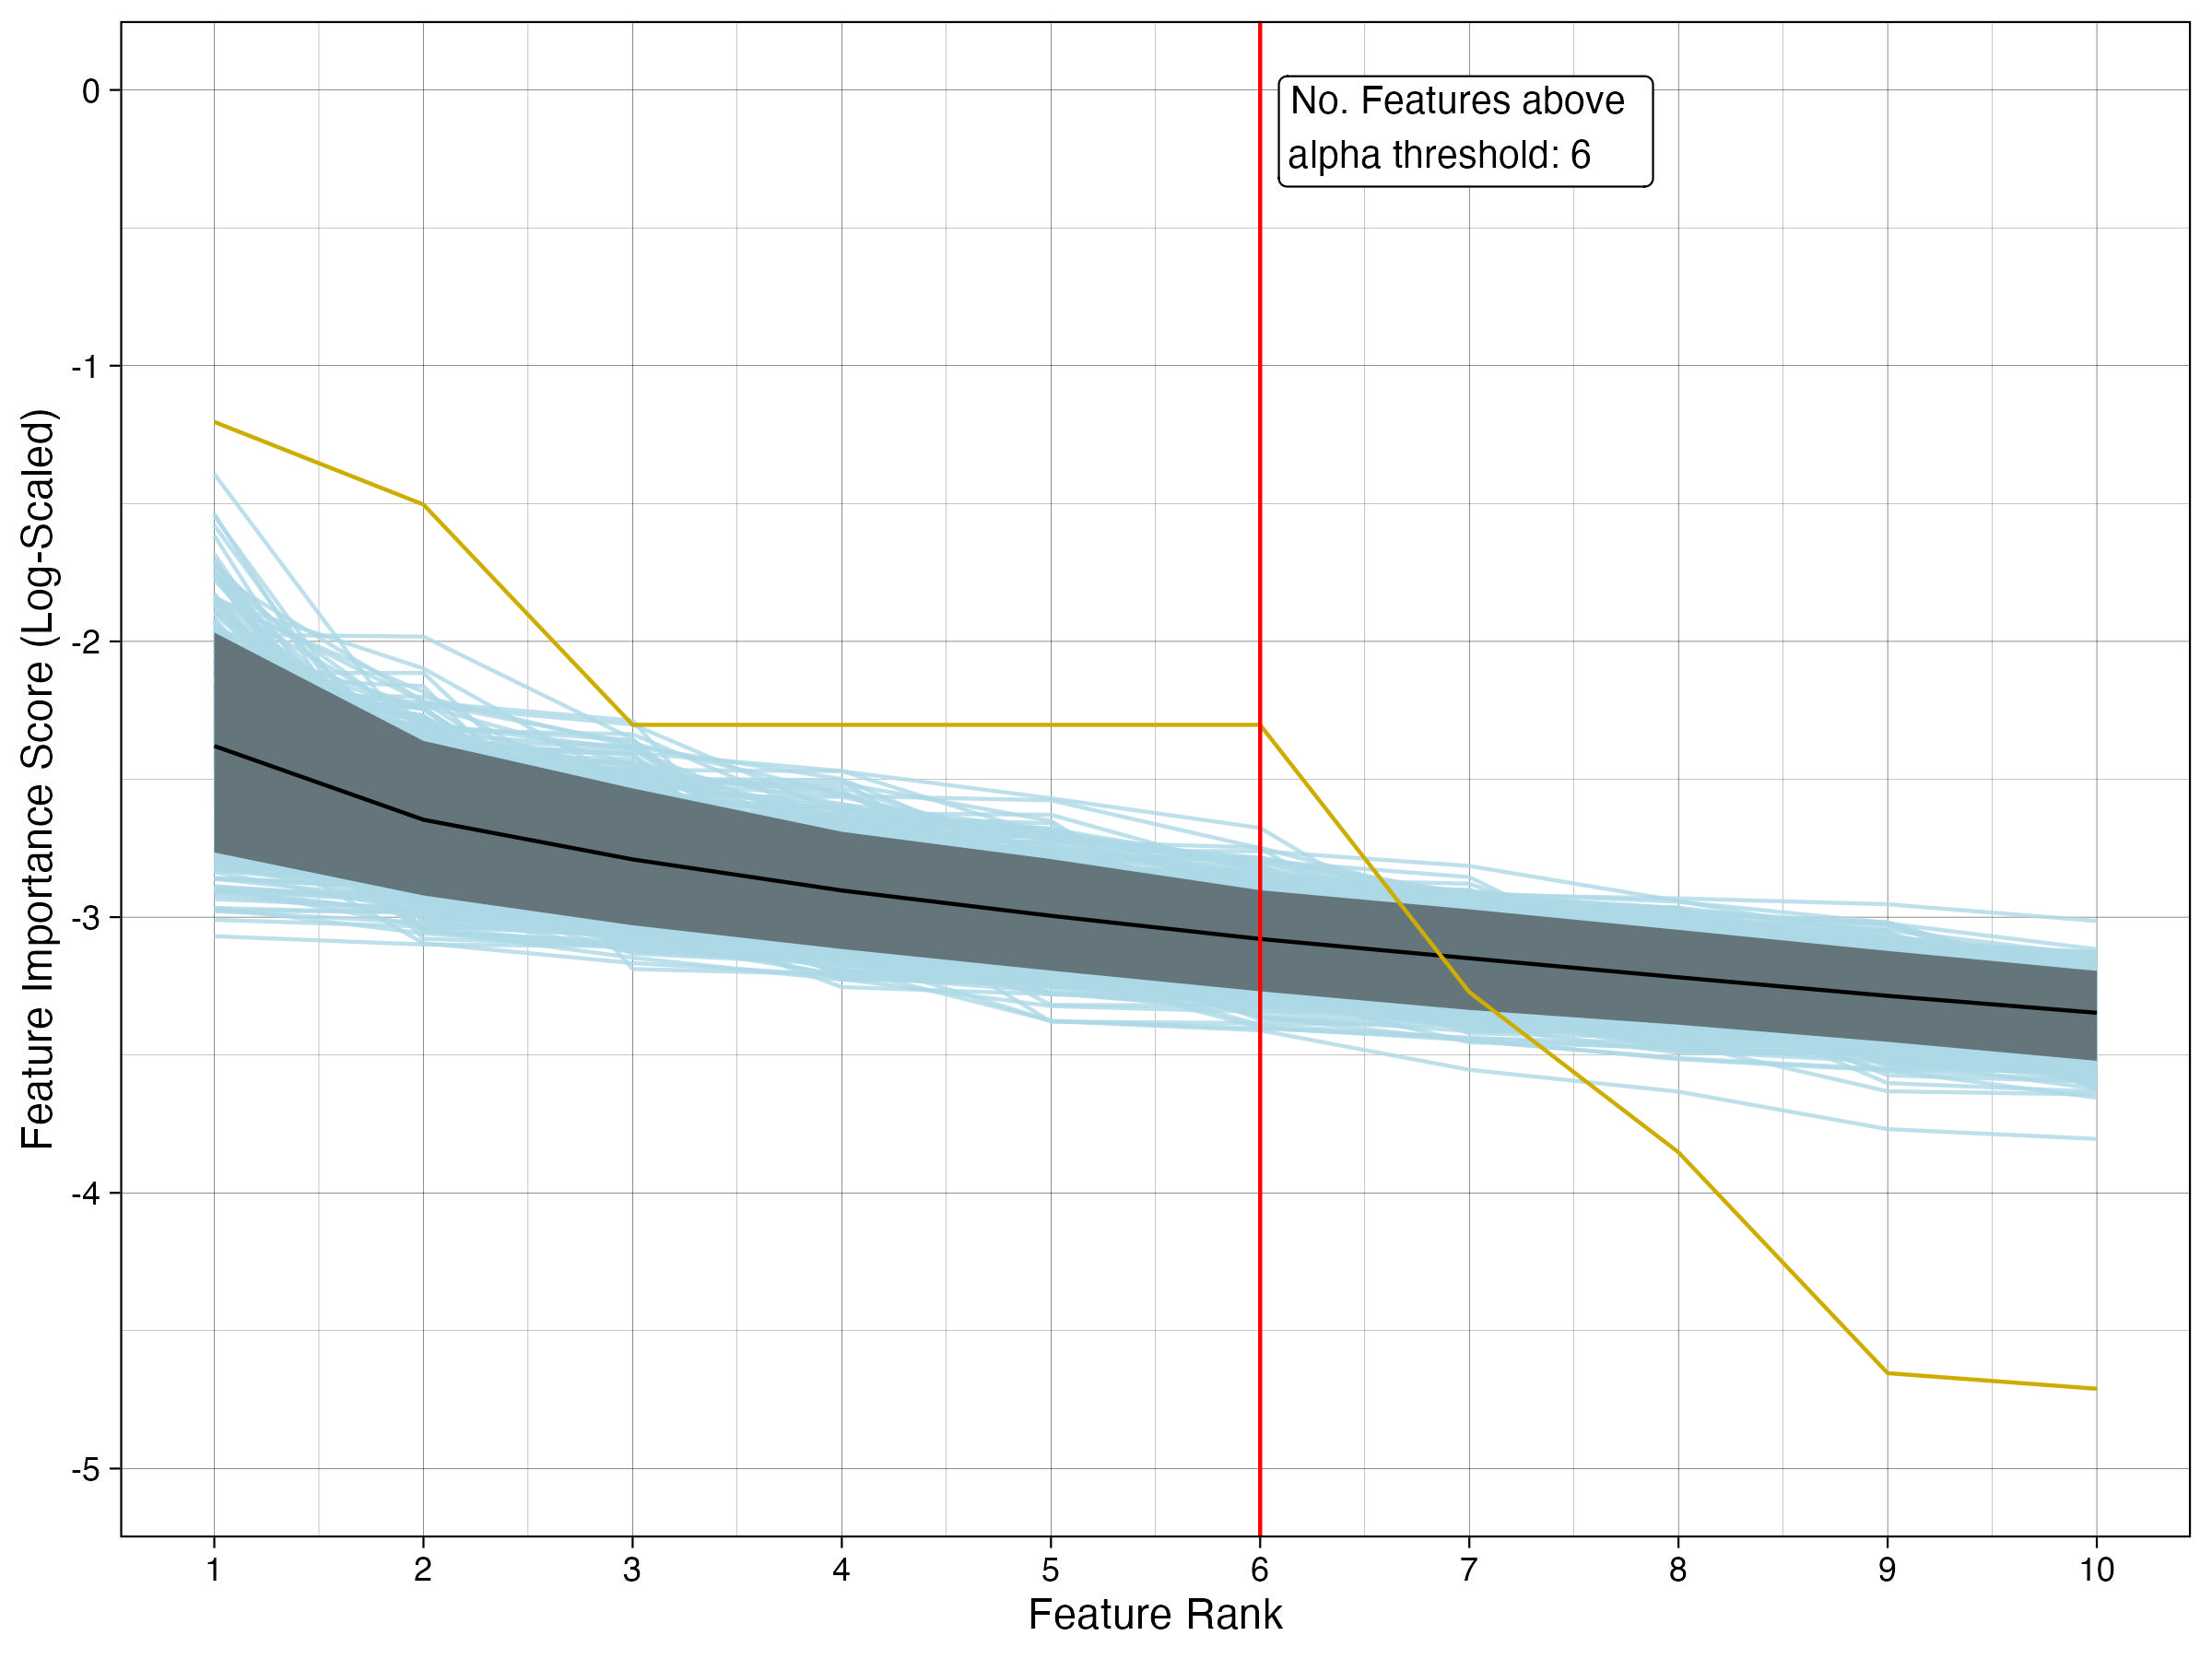
\includegraphics[width=1\linewidth]{images/demo_fiplot_full} \end{center}

\begin{Shaded}
\begin{Highlighting}[]
\CommentTok{\# Same plot as above, but zoomed to show only the significant results}
\NormalTok{fiplot\_focused }\OtherTok{\textless{}{-}}\NormalTok{ Rf2pval}\SpecialCharTok{::}\FunctionTok{generate\_fi\_rank\_plot}\NormalTok{(}
  \AttributeTok{permutedvalues =}\NormalTok{ feat\_importances}\SpecialCharTok{$}\NormalTok{permuted\_importances, }
  \AttributeTok{quantiledata =}\NormalTok{ quantile\_data, }
  \AttributeTok{xlimitmin =} \DecValTok{1}\NormalTok{, }
  \AttributeTok{xlimitmax =} \DecValTok{10}\NormalTok{, }
  \AttributeTok{ylimitmin=} \SpecialCharTok{{-}}\DecValTok{5}\NormalTok{, }
  \AttributeTok{ylimitmax =} \DecValTok{0}\NormalTok{, }
  \AttributeTok{labelhorizontaladjust =} \FloatTok{1.05}\NormalTok{,}
  \AttributeTok{labelverticaladjust =} \FloatTok{1.5}\NormalTok{,}
  \AttributeTok{focusedView =} \ConstantTok{TRUE}\NormalTok{,}
  \AttributeTok{logOn =} \ConstantTok{TRUE}
\NormalTok{  )}

\FunctionTok{print}\NormalTok{(fiplot\_focused)}
\end{Highlighting}
\end{Shaded}

\begin{center}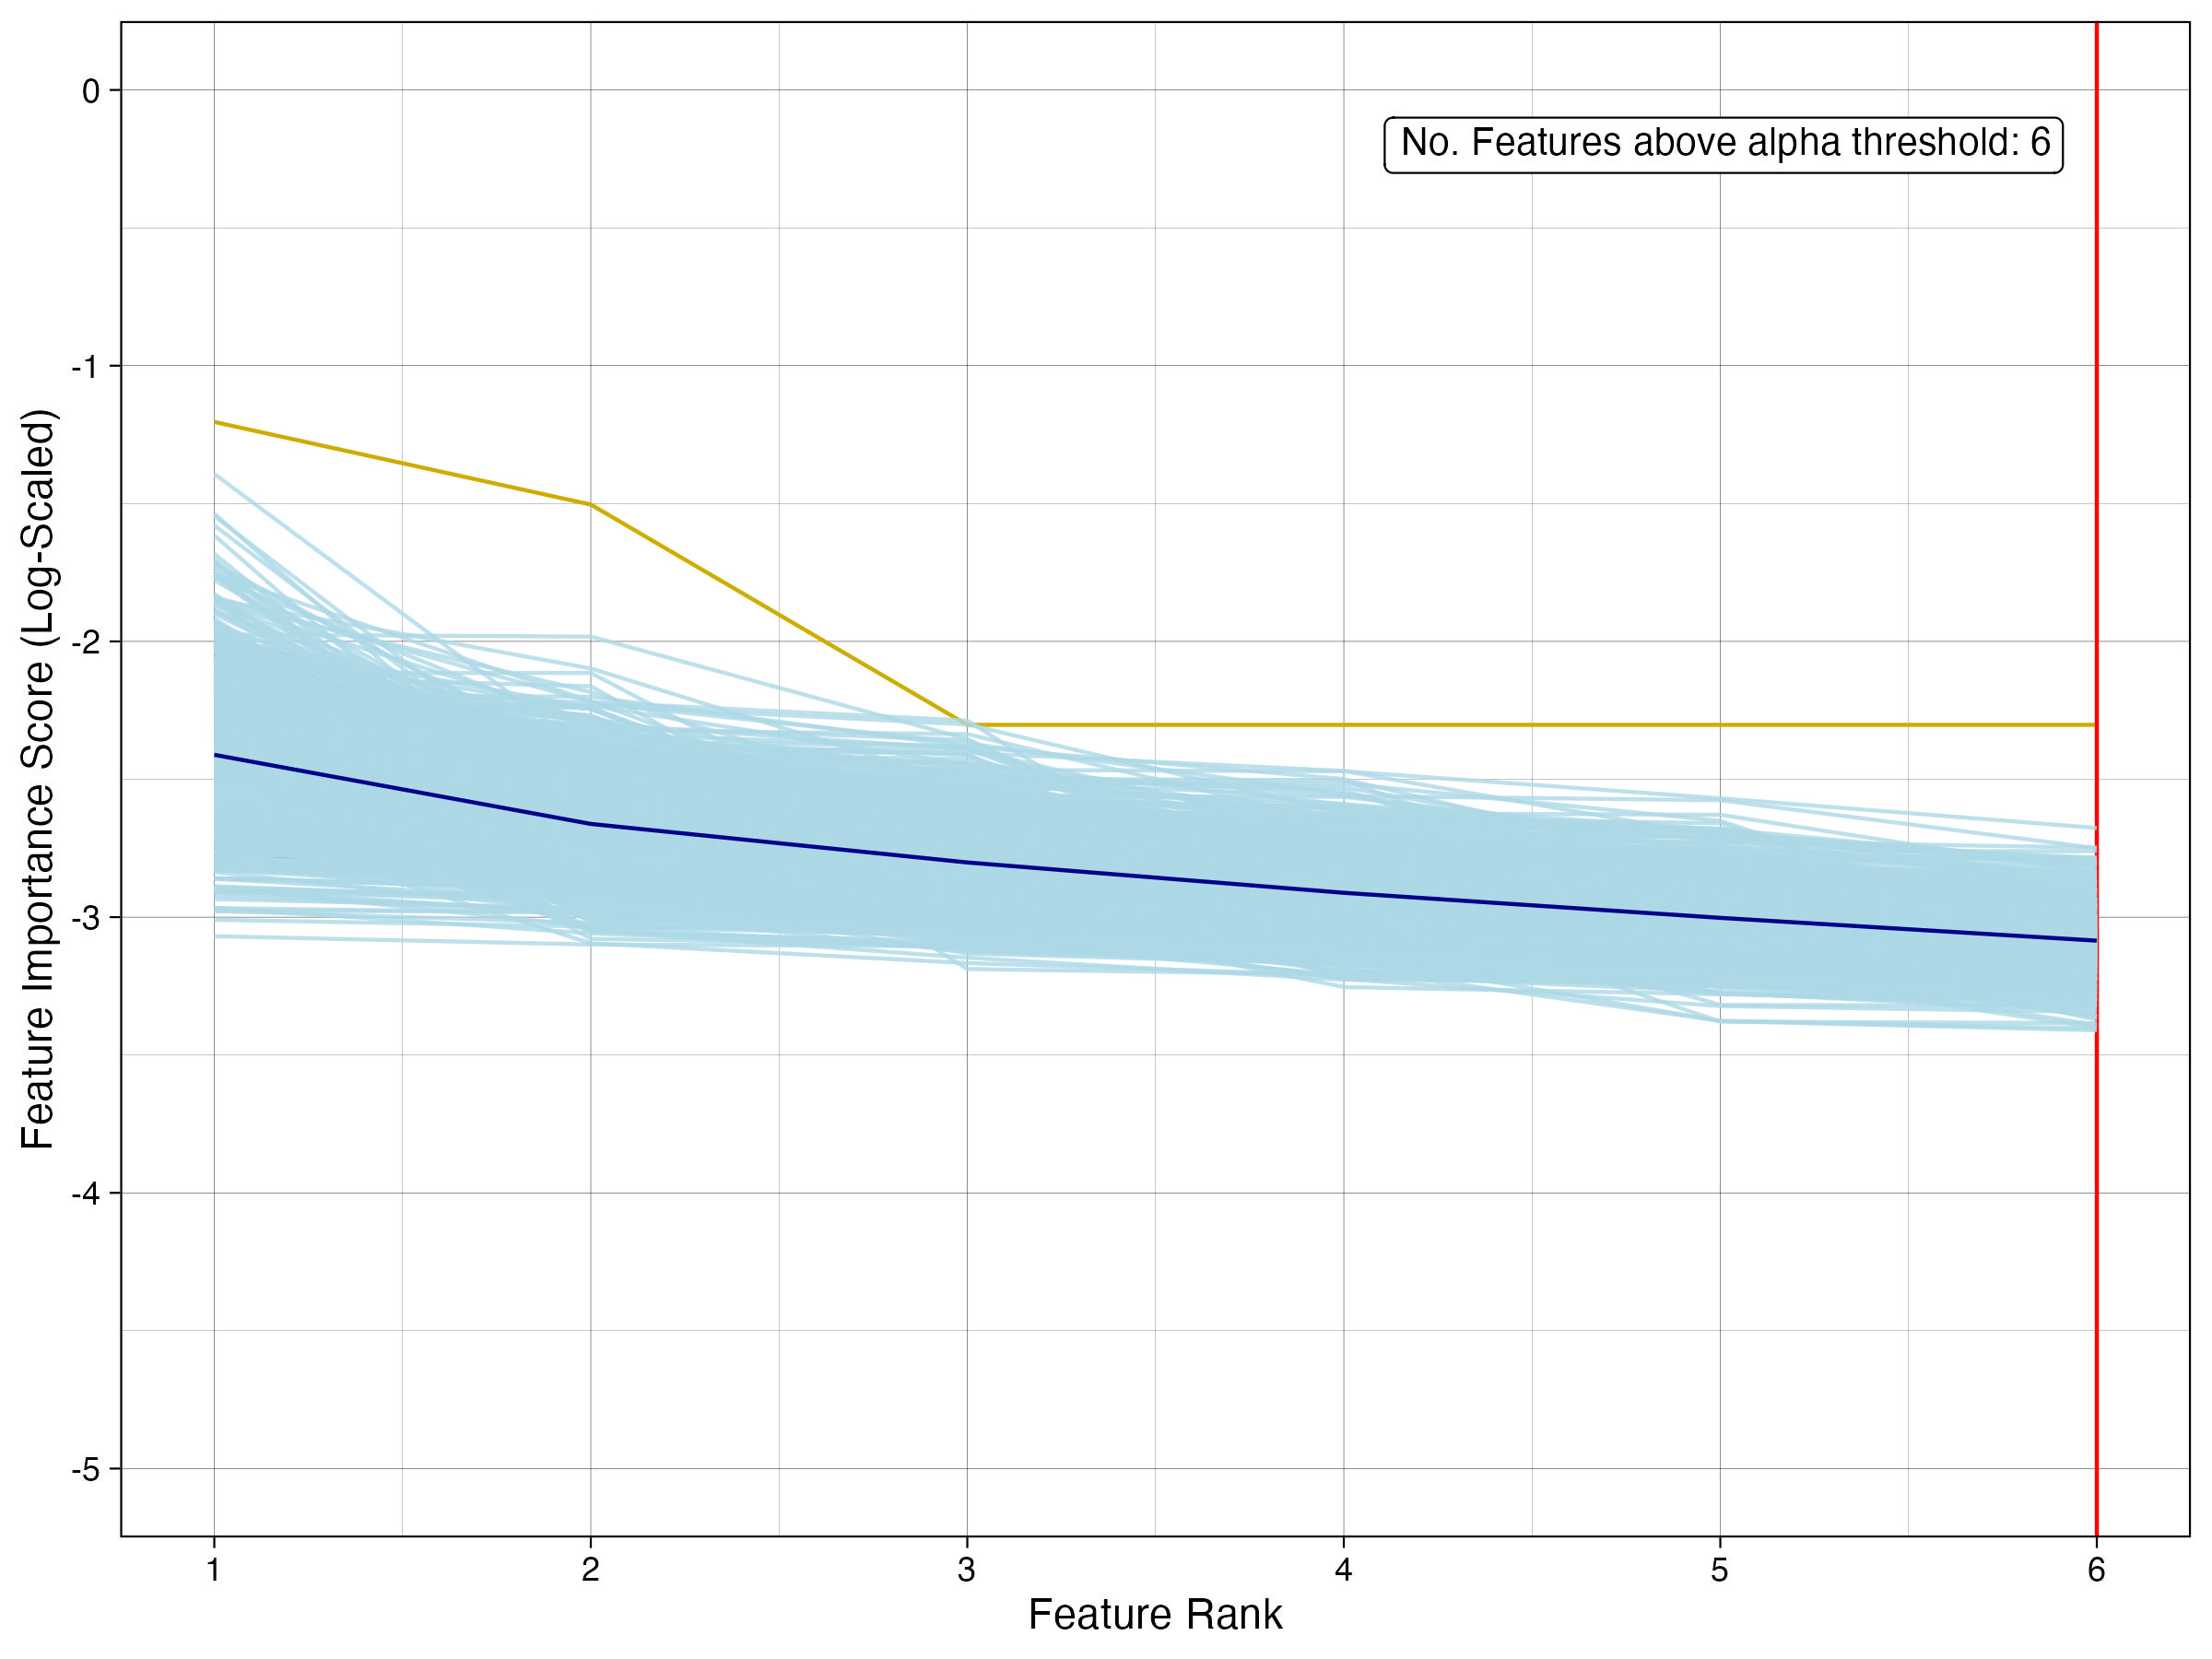
\includegraphics[width=1\linewidth]{images/demo_fiplot_focused} \end{center}

\hypertarget{pi-histogram}{%
\subsection{pi Histogram}\label{pi-histogram}}

\begin{Shaded}
\begin{Highlighting}[]
\CommentTok{\# Generate pi Histogram plot}
\CommentTok{\# Creates a histogram showing the sum of absolute deviations by count, the measures }
\CommentTok{\# used to calculate the pi statistics used in the p{-}value calculation for the set.}
\NormalTok{pihist\_plot }\OtherTok{\textless{}{-}}\NormalTok{ Rf2pval}\SpecialCharTok{::}\FunctionTok{generate\_pi\_histogram}\NormalTok{(}
  \AttributeTok{permutedvalues =}\NormalTok{ feat\_importances}\SpecialCharTok{$}\NormalTok{permuted\_importances, }
  \AttributeTok{quantiledata =}\NormalTok{ quantile\_data}
\NormalTok{  )}

\FunctionTok{print}\NormalTok{(pihist\_plot)}
\end{Highlighting}
\end{Shaded}

\begin{center}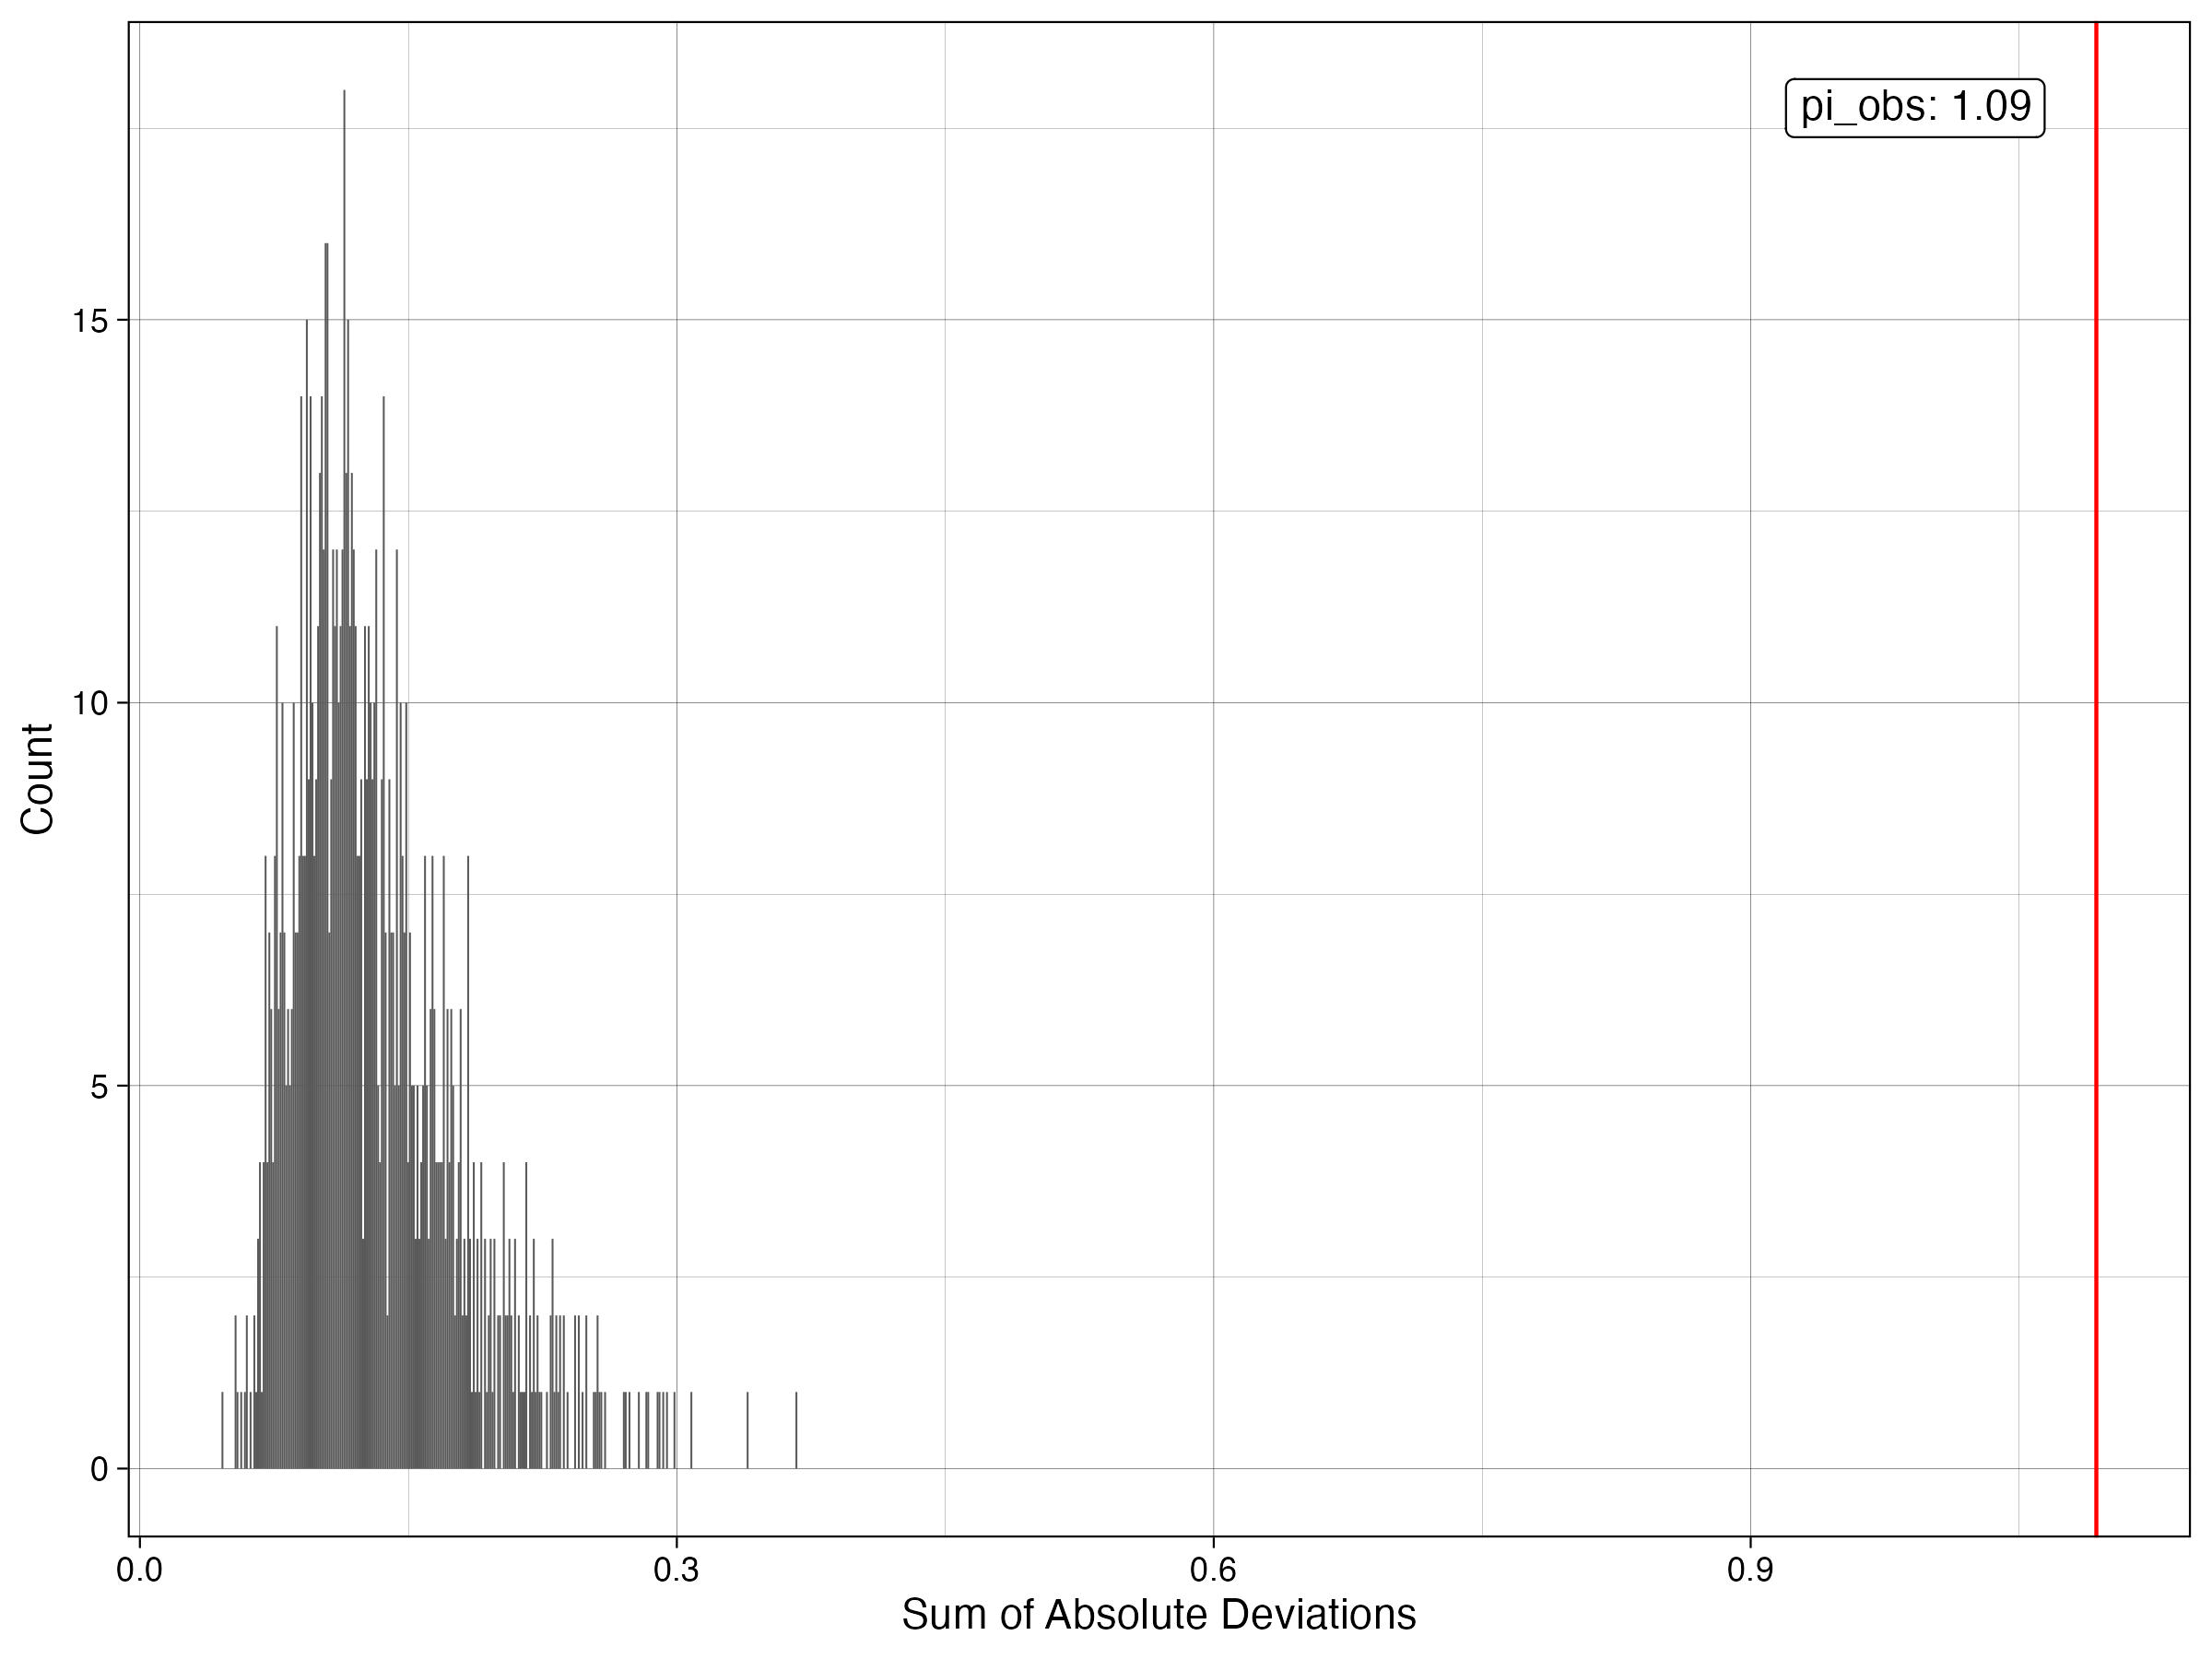
\includegraphics[width=1\linewidth]{images/demo_pihist_plot} \end{center}

\hypertarget{ecdf-plot}{%
\subsection{ECDF Plot}\label{ecdf-plot}}

\begin{Shaded}
\begin{Highlighting}[]
\CommentTok{\# Generate ECDF plot}
\CommentTok{\# Creates a plot of the empirical cumulative density function showing the sum of }
\CommentTok{\# absolute deviations by fraction of data.}
\NormalTok{ecdf\_plot }\OtherTok{\textless{}{-}}\NormalTok{ Rf2pval}\SpecialCharTok{::}\FunctionTok{generate\_pi\_ECDF\_plot}\NormalTok{(}
  \AttributeTok{permutedvalues =}\NormalTok{ feat\_importances}\SpecialCharTok{$}\NormalTok{permuted\_importances,}
  \AttributeTok{quantiledata =}\NormalTok{ quantile\_data)}

\FunctionTok{print}\NormalTok{(ecdf\_plot)}
\end{Highlighting}
\end{Shaded}

\begin{center}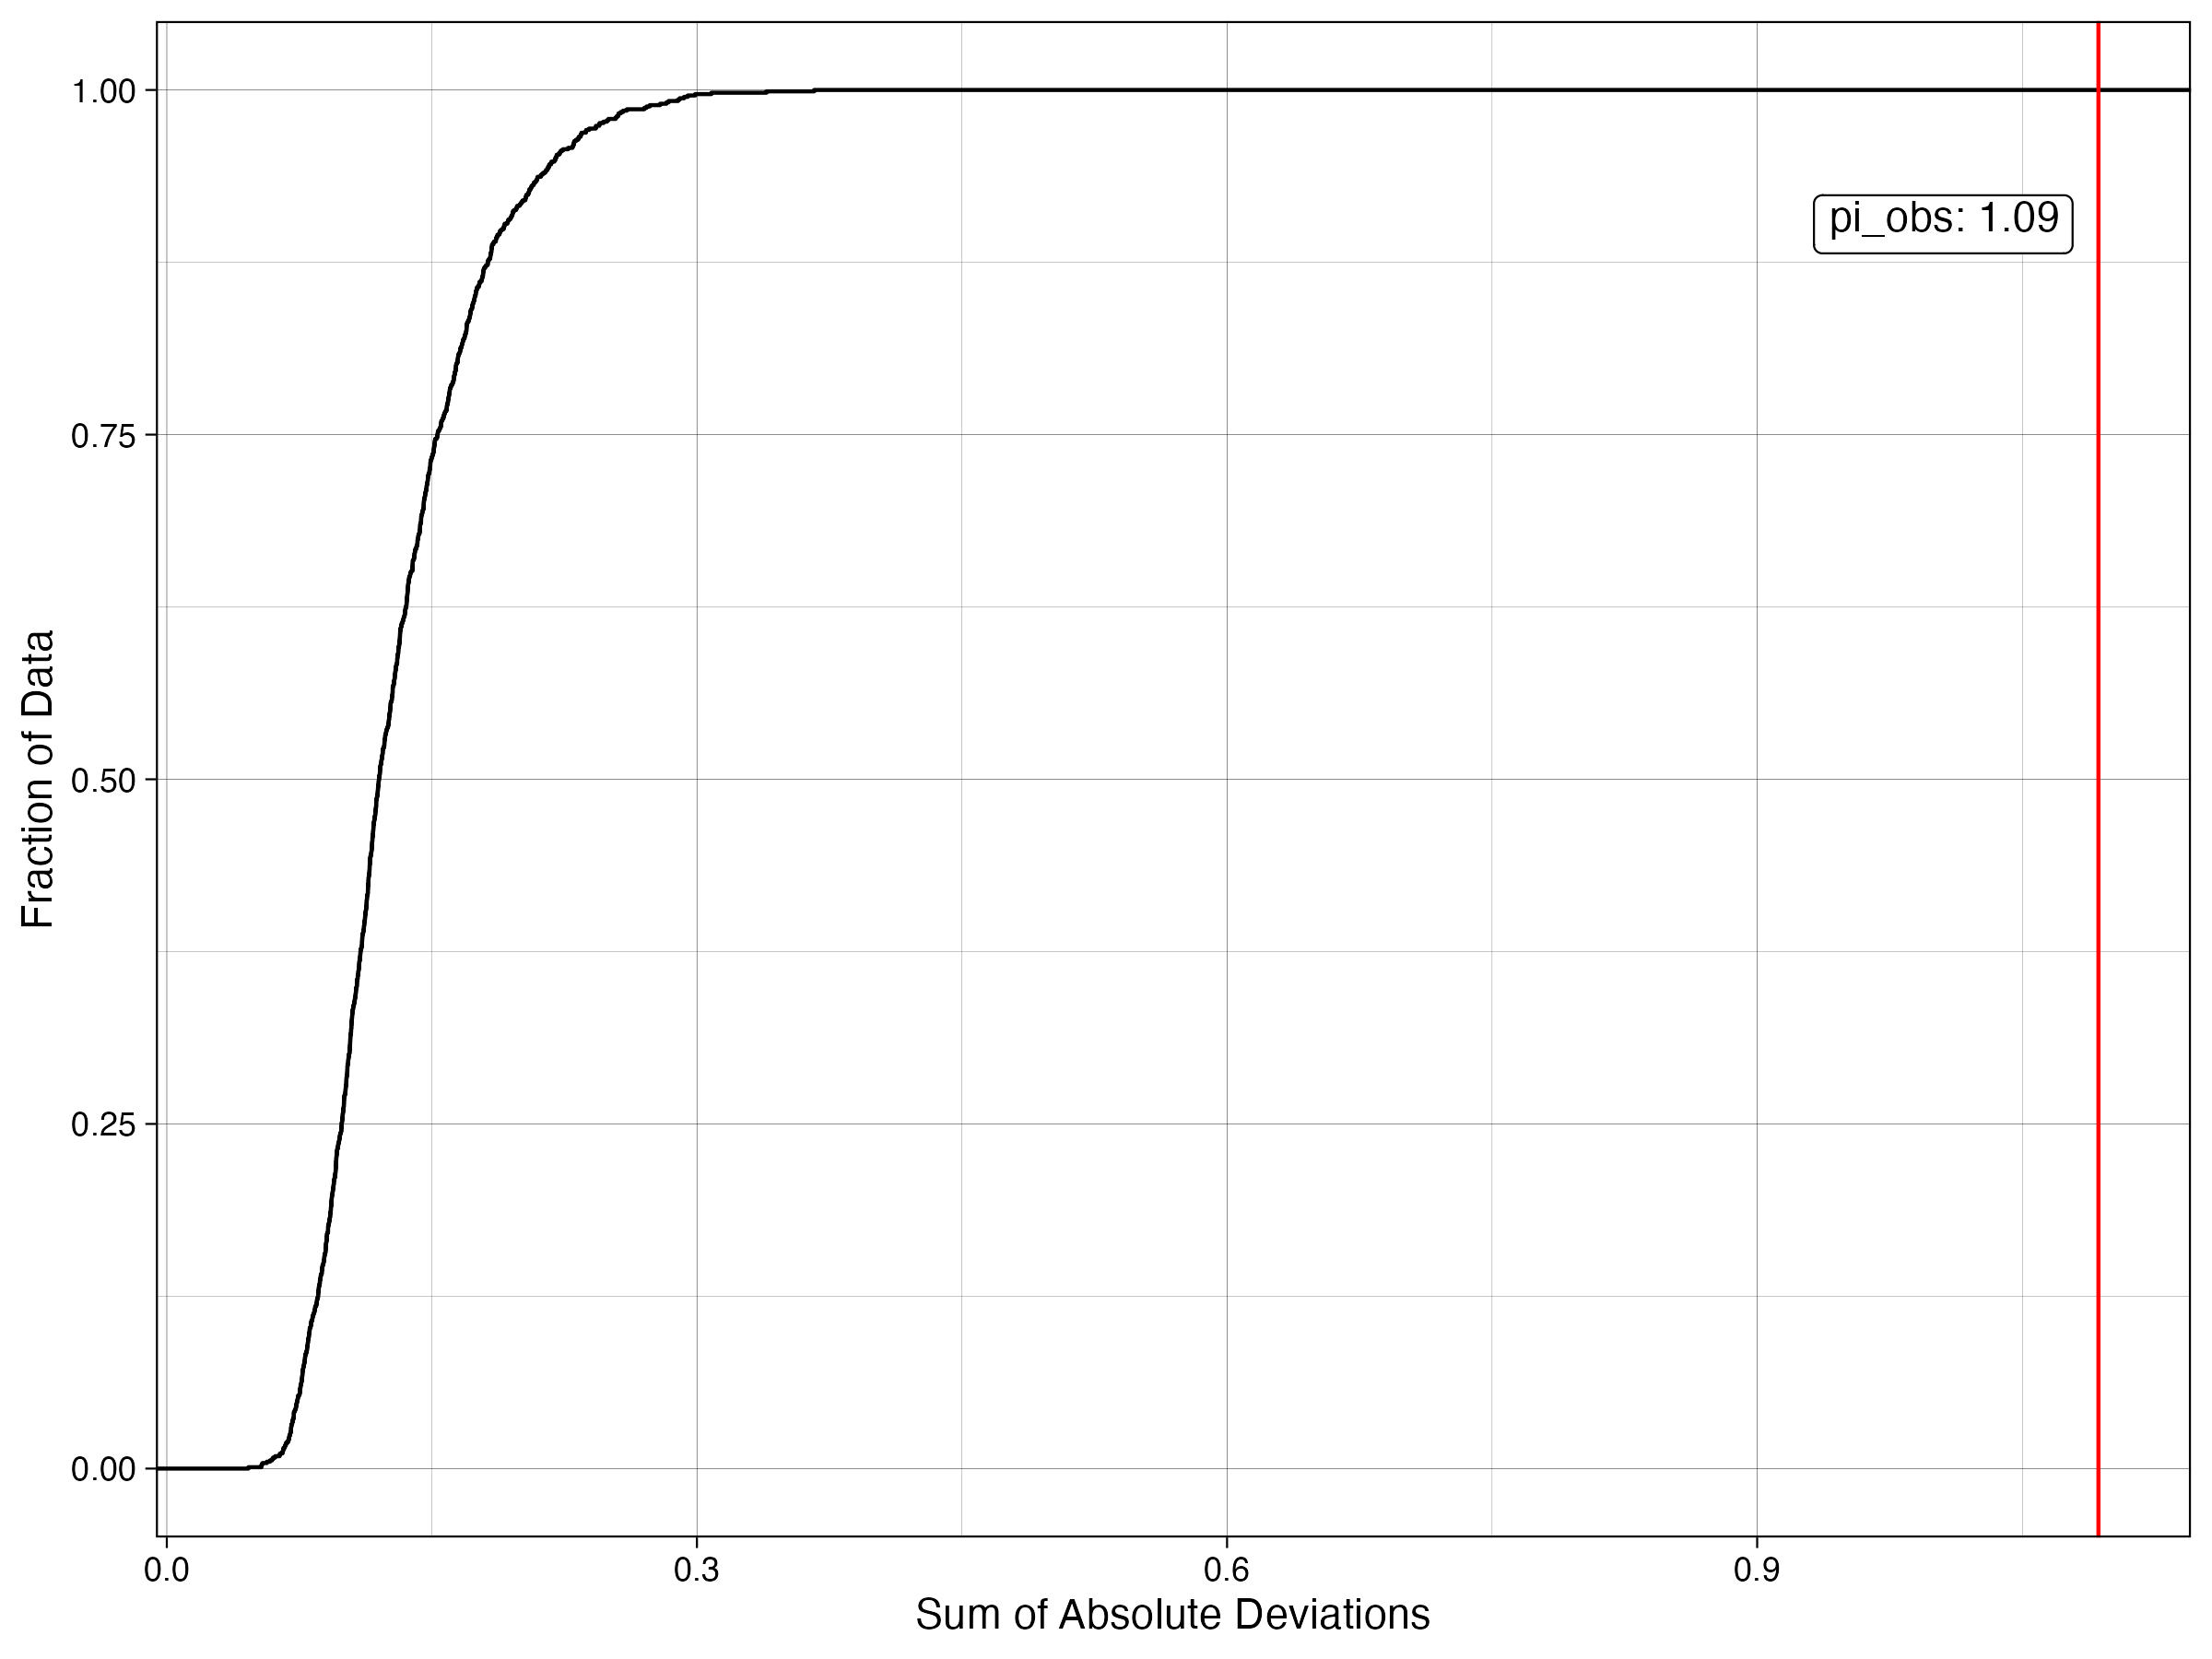
\includegraphics[width=1\linewidth]{images/demo_ecdf_plot} \end{center}

Advanced Features

Explore advanced functionalities of Rf2pval such as SHAP value analysis,
or use it to plug into additional gene ontology, enrichment and
gprofiler modules.

\hypertarget{shap-analysis}{%
\section{\texorpdfstring{\href{https://shap.readthedocs.io/en/latest/}{SHAP}
Analysis}{SHAP Analysis}}\label{shap-analysis}}

\begin{Shaded}
\begin{Highlighting}[]
\CommentTok{\# Produce a list of SHAP values}
\CommentTok{\# This function calculates SHAP values for a given dataset using a provided model. }
\CommentTok{\# It then identifies significant features based on the SHAP values for the specified class.}
\CommentTok{\# Additionally, it prepares a long{-}format data frame of individual SHAP values }
\CommentTok{\# suitable for visualization.}

\NormalTok{shapvals }\OtherTok{\textless{}{-}}\NormalTok{ Rf2pval}\SpecialCharTok{::}\FunctionTok{calculate\_SHAP\_values}\NormalTok{(}
  \AttributeTok{model =}\NormalTok{ fitting\_results}\SpecialCharTok{$}\NormalTok{model, }
  \AttributeTok{data =}\NormalTok{ processed\_training\_data}\SpecialCharTok{$}\NormalTok{X\_training\_mat, }
  \AttributeTok{class\_index =} \DecValTok{1}\NormalTok{, }\CommentTok{\# In demo, 1 represents Right}
  \AttributeTok{shap\_std\_dev\_factor =} \FloatTok{0.5}
\NormalTok{  )}

\CommentTok{\# Print the mapping list to remind of binary mapping and aid with SHAP plot }
\CommentTok{\# directionality interpretation.}
\CommentTok{\# If class\_index = 1, in the demo this represents the features contribution}
\CommentTok{\# towards the "Right". Thus in the plot \textquotesingle{}red\textquotesingle{} coloured features could be considered}
\CommentTok{\# to be positively contributing to "Right" side predictions, and \textquotesingle{}blue\textquotesingle{} coloured }
\CommentTok{\# features negatively to "Right" side predictions (or positively to "Left").}

\NormalTok{unique\_mapping }\OtherTok{\textless{}{-}}\FunctionTok{unique}\NormalTok{(demo\_rnaseq\_data}\SpecialCharTok{$}\NormalTok{target\_categories[, }\FunctionTok{c}\NormalTok{(}\StringTok{"target\_categorical"}\NormalTok{, }\StringTok{"target"}\NormalTok{)])}
\FunctionTok{print}\NormalTok{(unique\_mapping)}
 
\CommentTok{\# Produce the SHAP Plots}
\CommentTok{\# Generates a combined bar and beeswarm plot to show direction, }
\CommentTok{\# as well as global and local feature importances.}
\NormalTok{shapplot }\OtherTok{\textless{}{-}}\NormalTok{ Rf2pval}\SpecialCharTok{::}\FunctionTok{generate\_shap\_plots}\NormalTok{(}
  \AttributeTok{mean\_shap\_values =}\NormalTok{ shapvals}\SpecialCharTok{$}\NormalTok{significant\_features,}
  \AttributeTok{long\_shap\_data =}\NormalTok{ shapvals}\SpecialCharTok{$}\NormalTok{long\_shap\_data}
\NormalTok{  )}

\FunctionTok{print}\NormalTok{(shapplot)}
\end{Highlighting}
\end{Shaded}

\begin{center}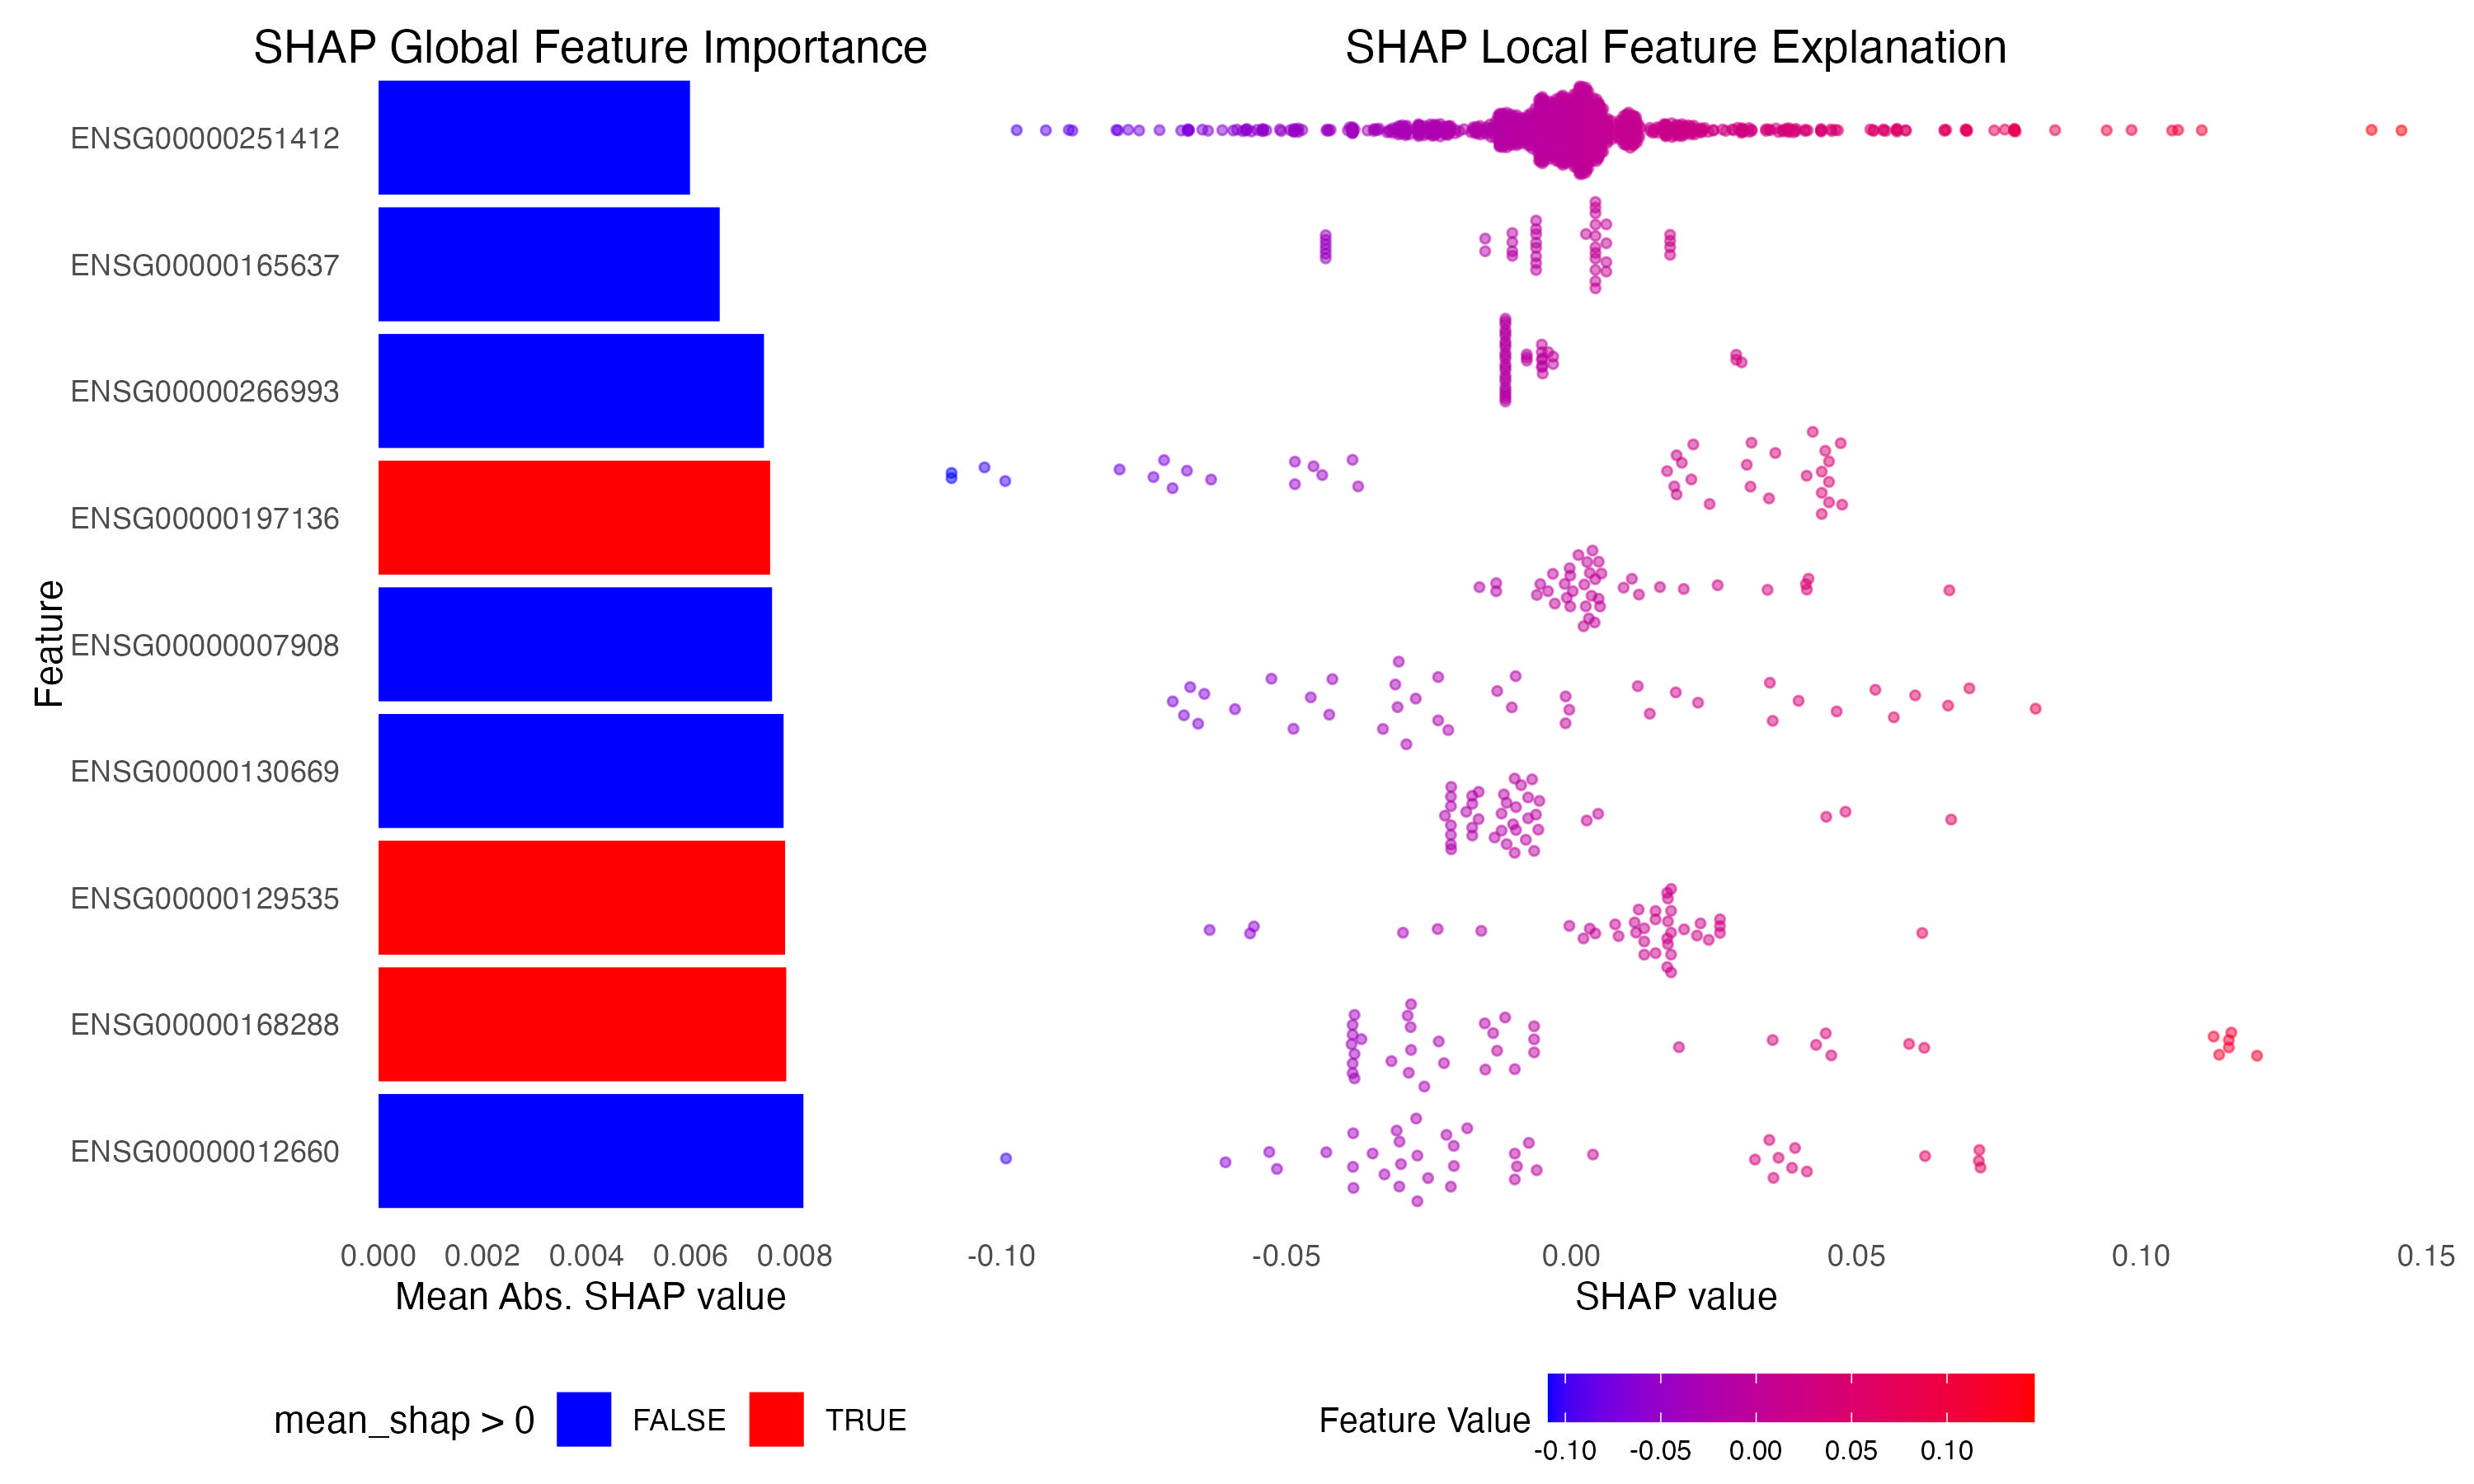
\includegraphics[width=1\linewidth]{images/demo_shap_plot_2_full} \end{center}

\hypertarget{go-enrichment-analysis}{%
\section{\texorpdfstring{\href{https://bioconductor.org/packages/release/bioc/html/clusterProfiler.html}{GO
Enrichment}
Analysis}{GO Enrichment Analysis}}\label{go-enrichment-analysis}}

\begin{Shaded}
\begin{Highlighting}[]
\FunctionTok{library}\NormalTok{(clusterProfiler)}
\FunctionTok{library}\NormalTok{(org.Hs.eg.db) }\CommentTok{\# Assuming human data, if not see bioconductor for other organism dbs.}
\FunctionTok{library}\NormalTok{(enrichplot)}

\CommentTok{\# We have 3 lists of significant features from our data that can be explored further}

\CommentTok{\# 1. The \textquotesingle{}raw\textquotesingle{} list of siginificant features from the RF model (pre{-}Rank based feature reduction):}
\FunctionTok{print}\NormalTok{(feat\_importances}\SpecialCharTok{$}\NormalTok{top\_features)}

\CommentTok{\# 2. The list of significant features after rank{-}based permutation feature reduction}
\CommentTok{\# This is the most conservative, statistically stringent list:}
\FunctionTok{print}\NormalTok{(pvalues\_ranks)}

\CommentTok{\# 3. The list of significant features from the SHAP analysis}
\CommentTok{\# Can be further divided by directionality +/{-}:}
\FunctionTok{print}\NormalTok{(shapvals}\SpecialCharTok{$}\NormalTok{significant\_features)}

\CommentTok{\# Subsequent steps can be ran on any of these feature lists,}
\CommentTok{\# although if the list is too small these steps may not produce results.}
\NormalTok{features\_list }\OtherTok{\textless{}{-}}\NormalTok{ shapvals}\SpecialCharTok{$}\NormalTok{significant\_features}\SpecialCharTok{$}\NormalTok{feature }\CommentTok{\# Features from SHAP}

\CommentTok{\# Alternatively:}
\CommentTok{\#features\_list \textless{}{-} pvalues\_ranks$feature \# Post{-}rank based feature reduction list}
\CommentTok{\#features\_list \textless{}{-} feat\_importances$top\_features \# Pre{-}feature reduction list}

\CommentTok{\# Run the GO Enrichment Analysis}
\CommentTok{\# From clusterProfiler: GO Enrichment Analysis of a gene set. }
\CommentTok{\# Given a vector of genes, this function will return the enrichment GO categories.}

\NormalTok{ego }\OtherTok{\textless{}{-}}\NormalTok{ clusterProfiler}\SpecialCharTok{::}\FunctionTok{enrichGO}\NormalTok{(}
                \AttributeTok{gene =}\NormalTok{ features\_list,}
                \AttributeTok{OrgDb =}\NormalTok{ org.Hs.eg.db,}
                \AttributeTok{keyType =} \StringTok{"ENSEMBL"}\NormalTok{,}
                \AttributeTok{ont =} \StringTok{"ALL"}\NormalTok{, }\CommentTok{\# consider BP, CC, and MF ontologies}
                \AttributeTok{pAdjustMethod =} \StringTok{"BH"}\NormalTok{, }\CommentTok{\# adjust p{-}values for multiple testing}
                \AttributeTok{readable =} \ConstantTok{TRUE}\NormalTok{)  }\CommentTok{\# convert Entrez IDs back to gene symbols}

\CommentTok{\# Plot the gene ontology}
\NormalTok{enrich\_plot }\OtherTok{\textless{}{-}}\NormalTok{ enrichplot}\SpecialCharTok{::}\FunctionTok{dotplot}\NormalTok{(ego, }\AttributeTok{showCategory=}\DecValTok{20}\NormalTok{) }\SpecialCharTok{+} 
                                      \FunctionTok{ggtitle}\NormalTok{(}\StringTok{"Gene Ontology for Top Features"}\NormalTok{)}
\FunctionTok{print}\NormalTok{(enrich\_plot)}
\end{Highlighting}
\end{Shaded}

\begin{center}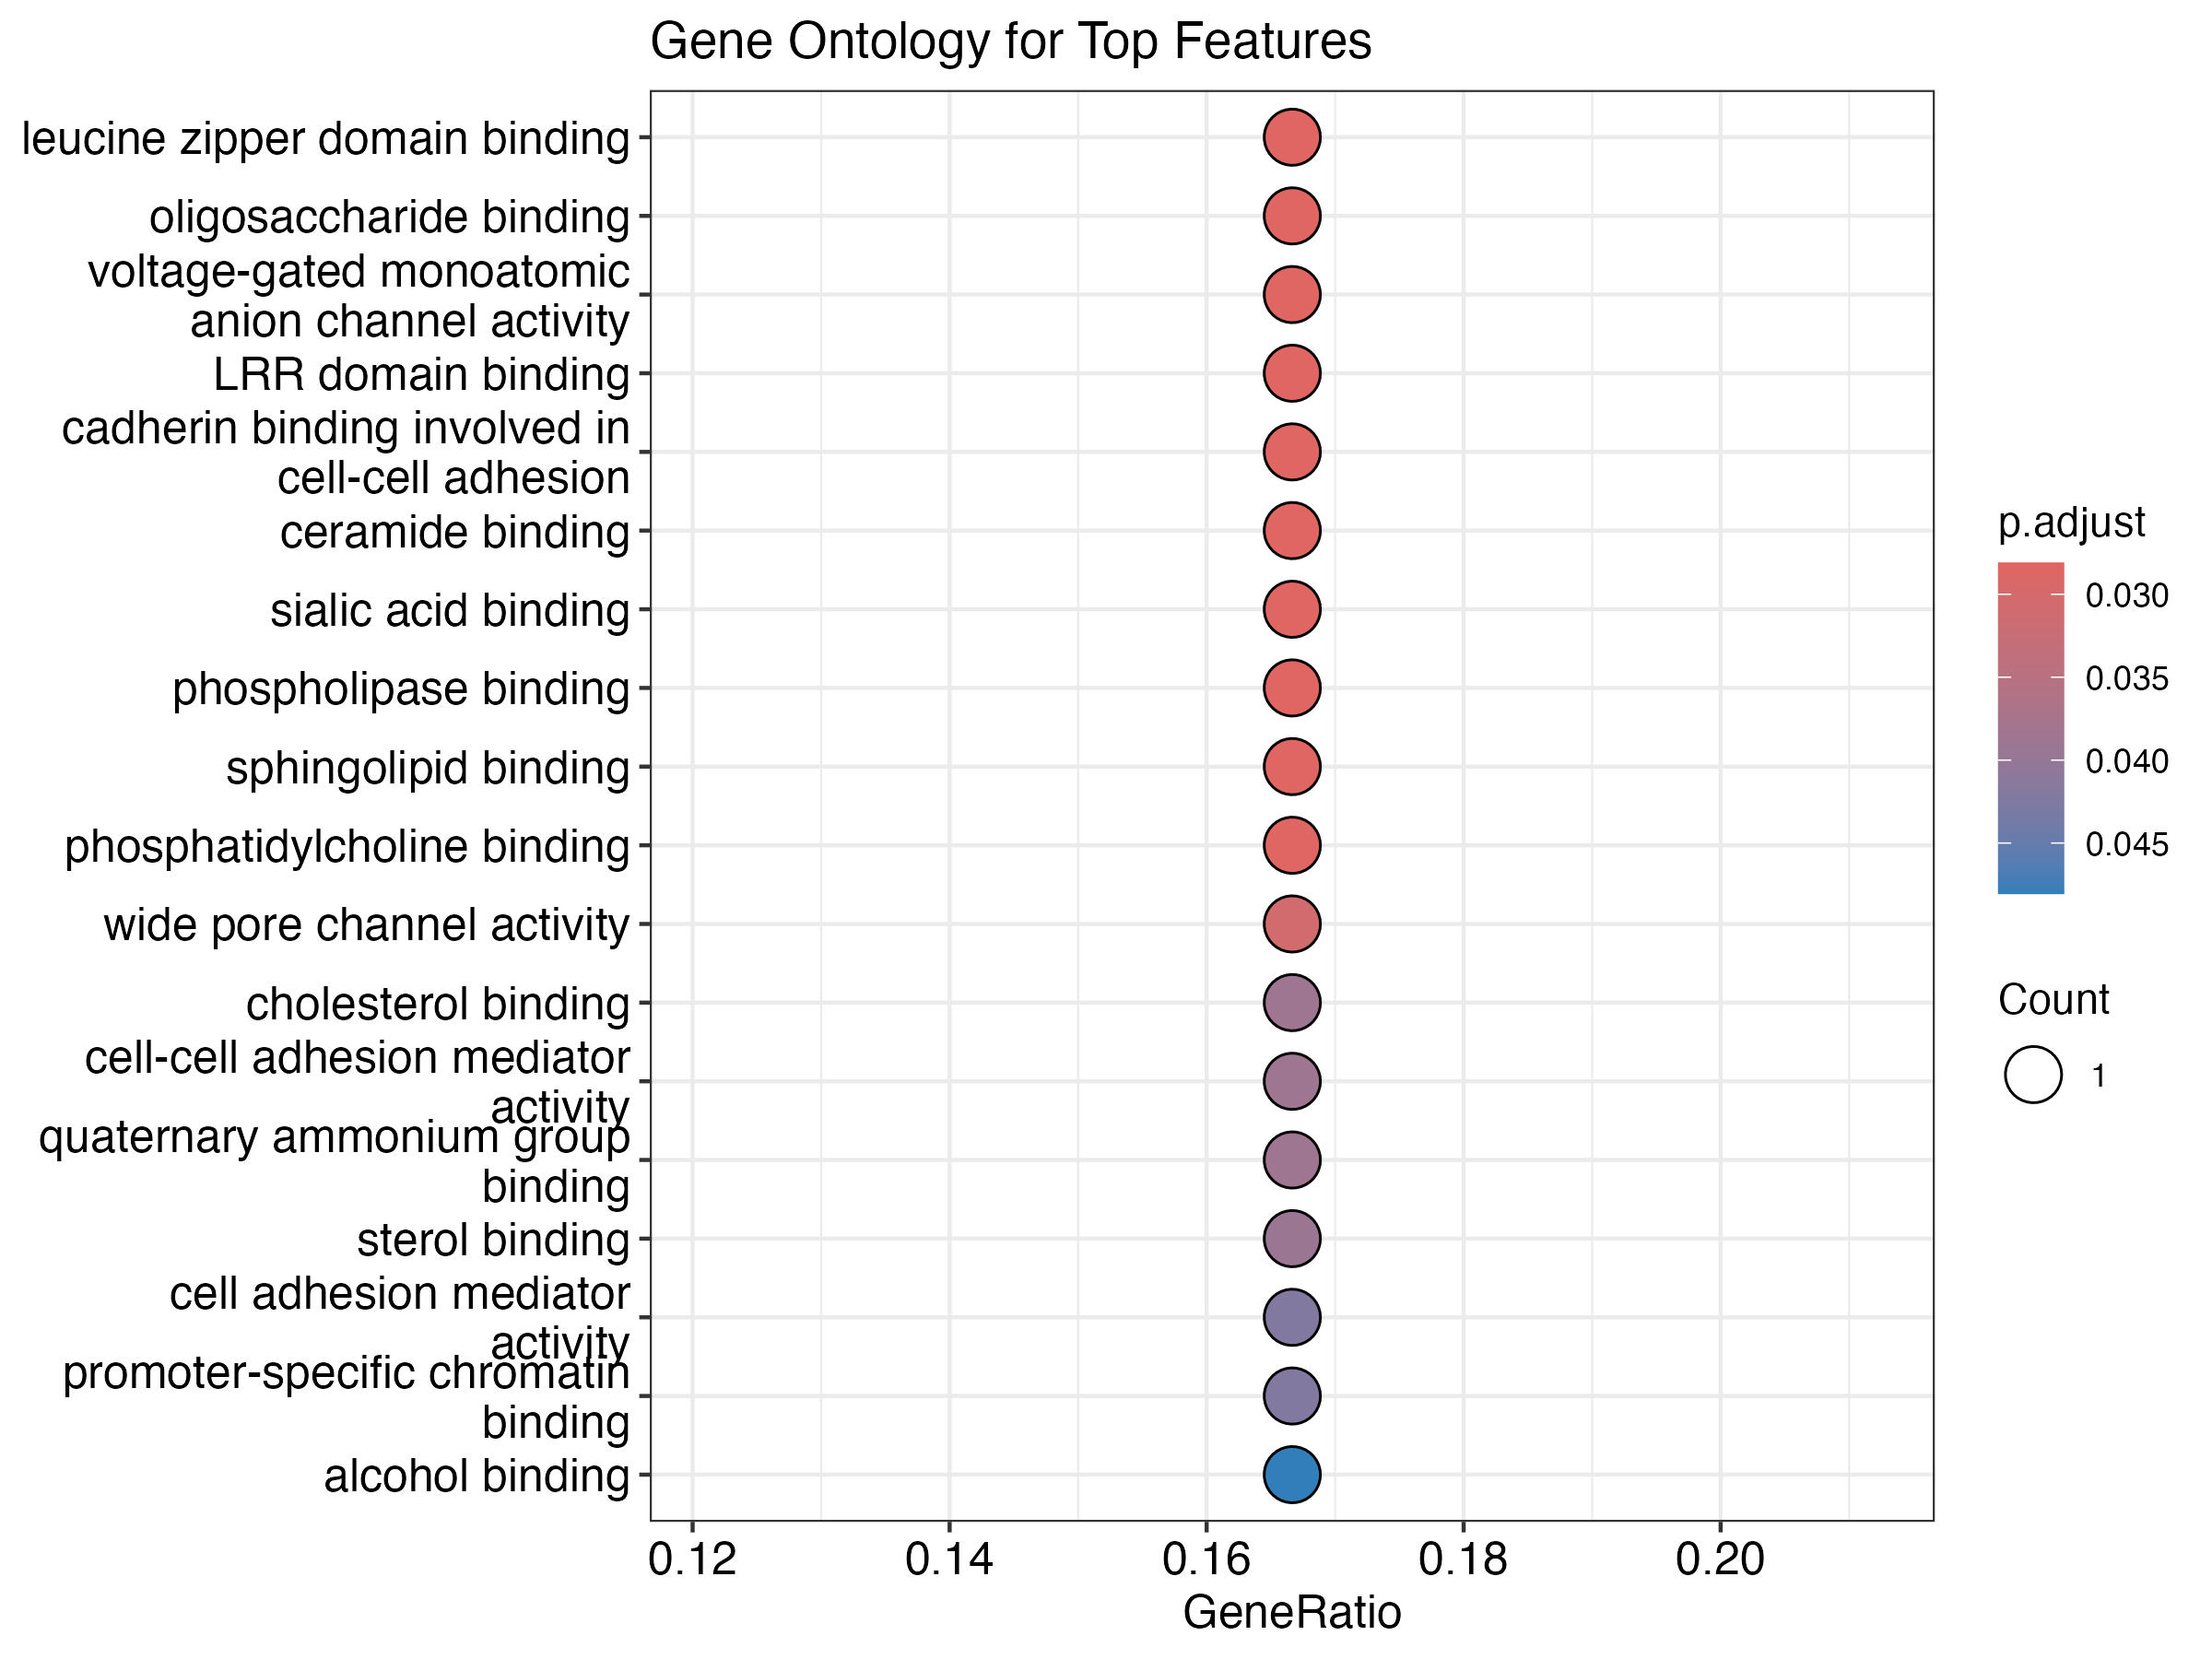
\includegraphics[width=1\linewidth]{images/demo_enrich_plot} \end{center}

\hypertarget{gprofiler-analysis}{%
\section{\texorpdfstring{\href{https://biit.cs.ut.ee/gprofiler/gost}{gProfiler}
Analysis}{gProfiler Analysis}}\label{gprofiler-analysis}}

\begin{Shaded}
\begin{Highlighting}[]
\FunctionTok{library}\NormalTok{(gprofiler2)}

\CommentTok{\# Perform the enrichment analysis}
\CommentTok{\# From gprofiler2: Interface to the g:Profiler tool g:GOSt }
\CommentTok{\# See https://biit.cs.ut.ee/gprofiler/gost for functional enrichments analysis of }
\CommentTok{\# gene lists.}

\NormalTok{gprofiler\_results }\OtherTok{\textless{}{-}}\NormalTok{ gprofiler2}\SpecialCharTok{::}\FunctionTok{gost}\NormalTok{(}\AttributeTok{query =}\NormalTok{ features\_list, }\CommentTok{\# List of gene vectors}
                                      \AttributeTok{organism =} \StringTok{"hsapiens"}\NormalTok{, }
                                      \AttributeTok{ordered\_query =} \ConstantTok{FALSE}\NormalTok{, }
                                      \AttributeTok{user\_threshold =} \FloatTok{0.5}
\NormalTok{                                      )}

\CommentTok{\# Create gProfiler Manhattan plot}
\CommentTok{\# From gprofiler2: This function creates a Manhattan plot out of the results from the }
\CommentTok{\# gprofiler2::gost() function. }
\NormalTok{gostplot\_mh\_plot }\OtherTok{\textless{}{-}}\NormalTok{ gprofiler2}\SpecialCharTok{::}\FunctionTok{gostplot}\NormalTok{(}\AttributeTok{gostres =}\NormalTok{ gprofiler\_results, }
                                         \AttributeTok{capped =} \ConstantTok{FALSE}\NormalTok{, }
                                         \AttributeTok{interactive =}\NormalTok{ F}
\NormalTok{                                         )}

\FunctionTok{print}\NormalTok{(gostplot\_mh\_plot)}
\end{Highlighting}
\end{Shaded}

\begin{center}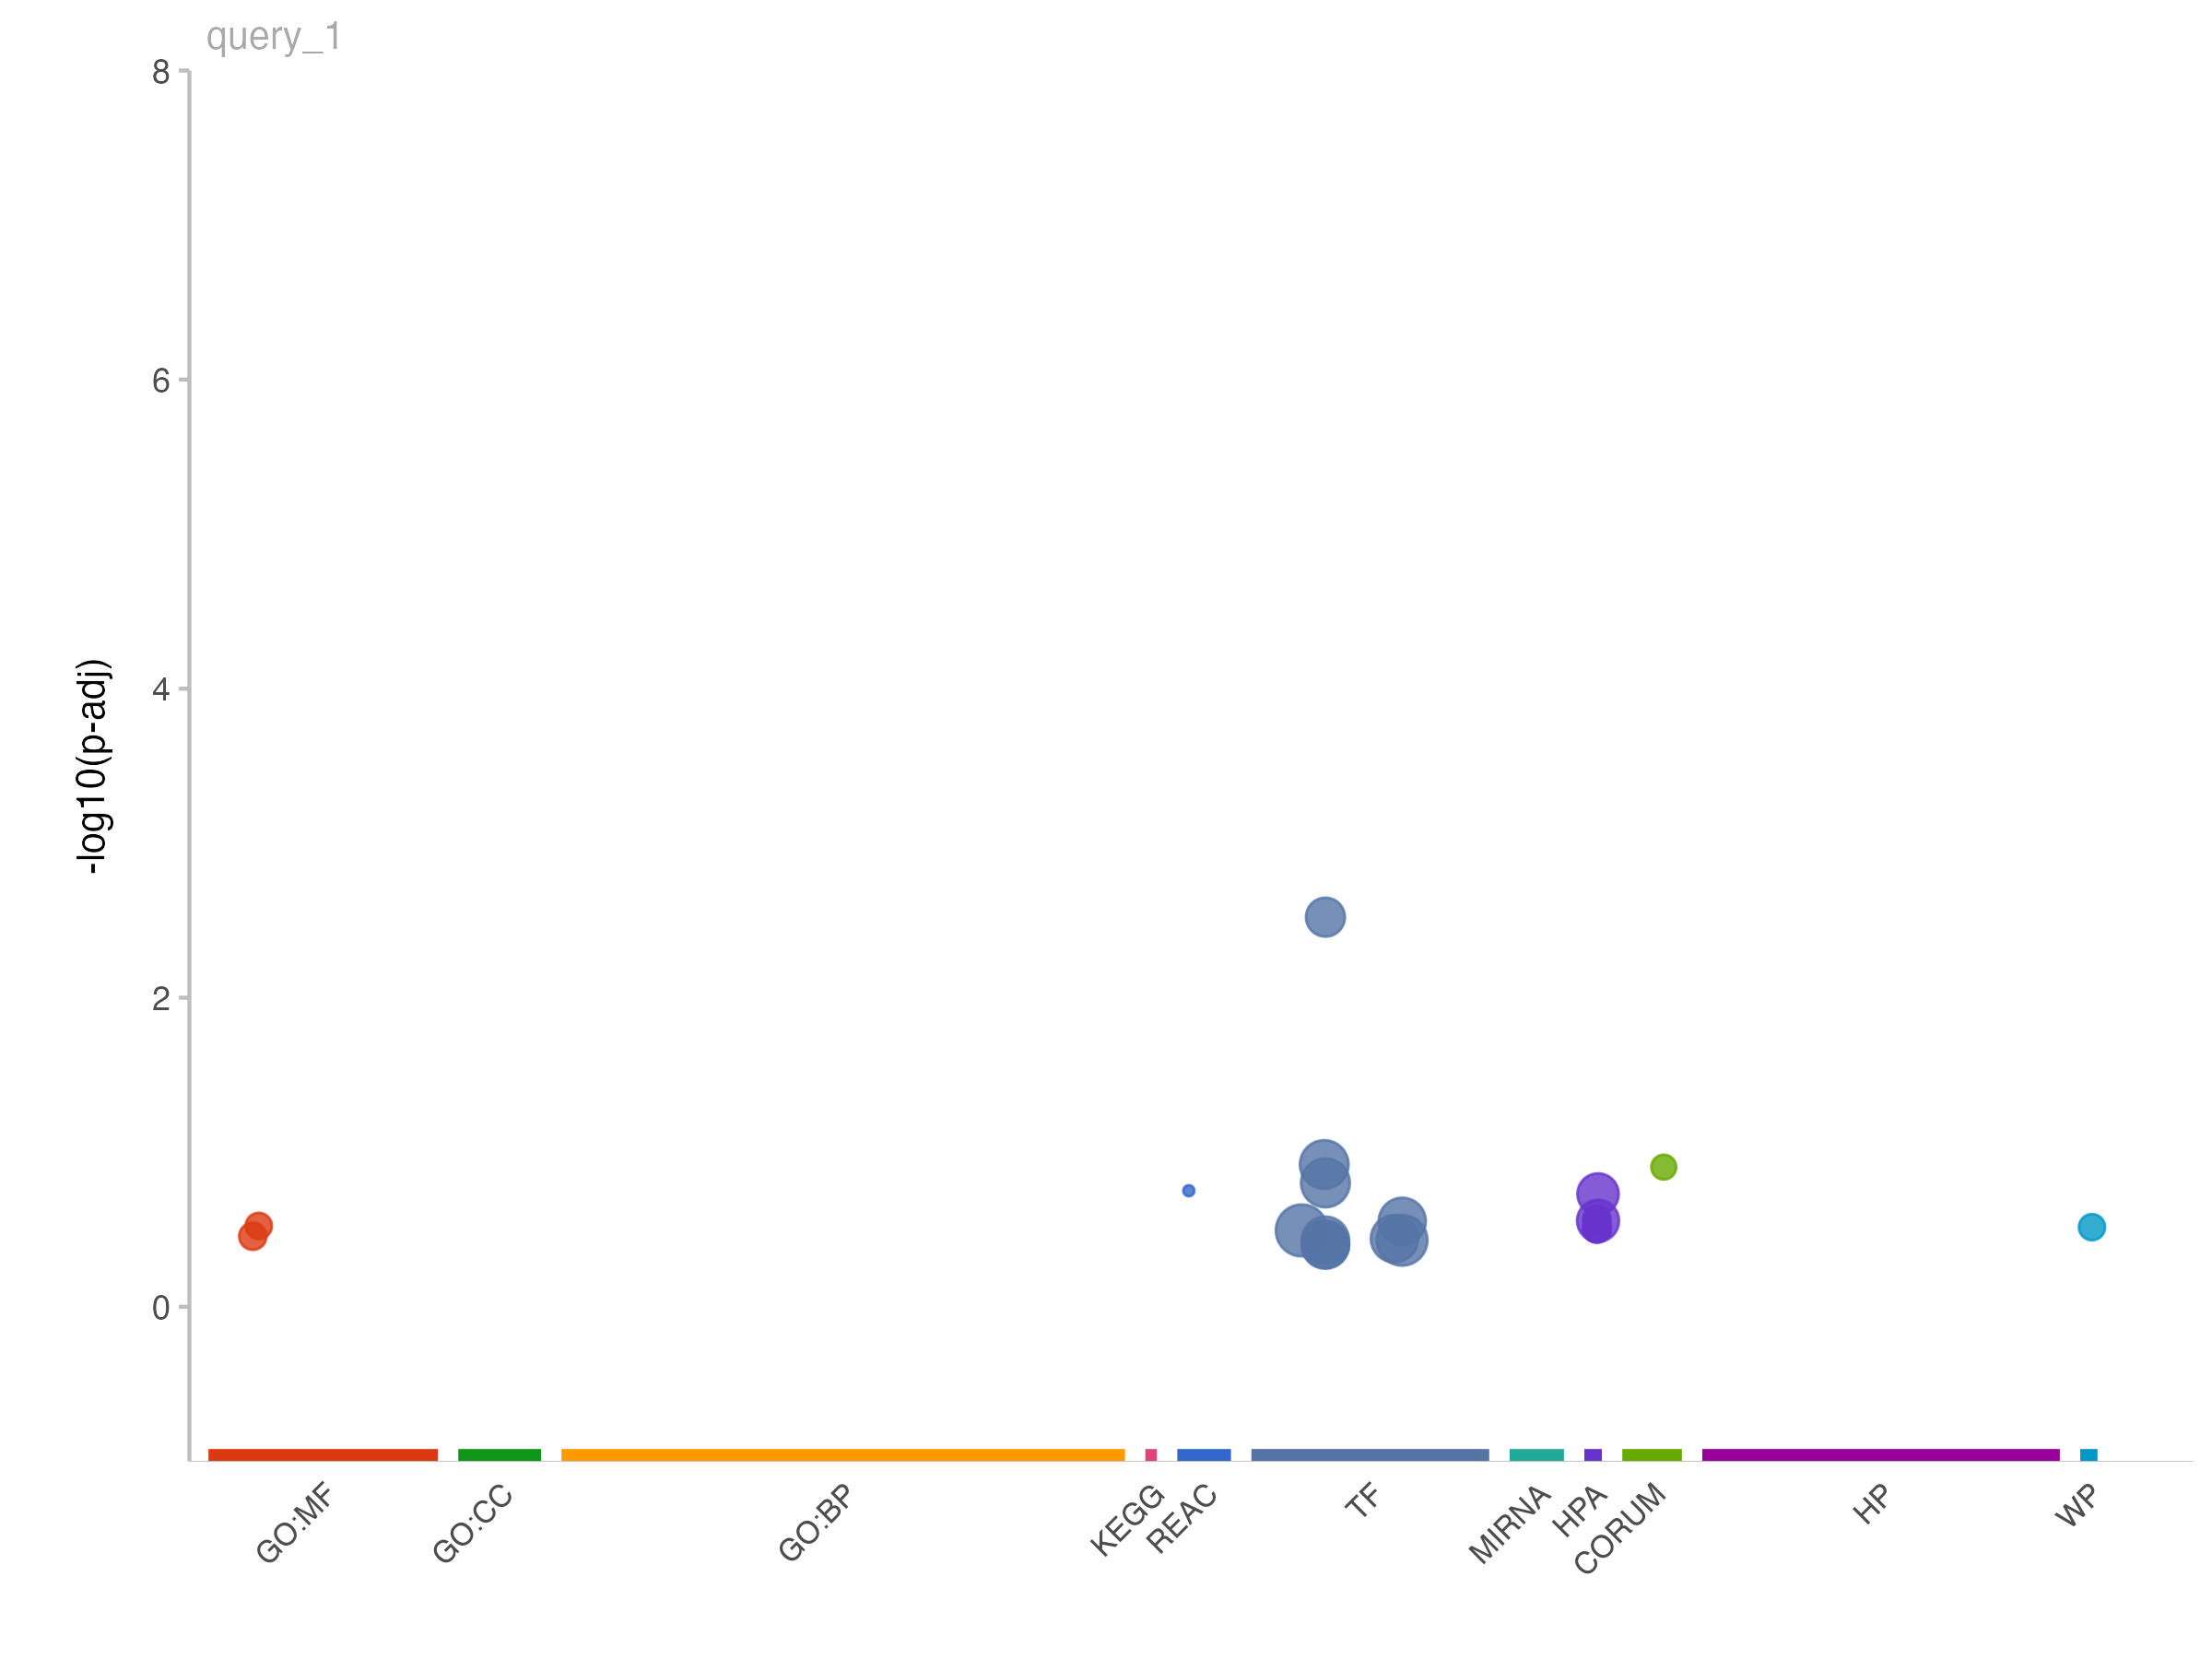
\includegraphics[width=1\linewidth]{images/demo_gostplot_mhplot} \end{center}

\begin{Shaded}
\begin{Highlighting}[]
\CommentTok{\# Create gProfiler Manhattan plot with table of terms beneath it}
\CommentTok{\# From gprofiler2: This function allows to highlight a list of selected terms on the }
\CommentTok{\# Manhattan plot created with the gprofiler2::gostplot() function. The resulting plot}
\CommentTok{\# is saved to a publication ready image if \textquotesingle{}filename\textquotesingle{} is specified. }
\CommentTok{\# The plot is very similar to the one shown in the g:GOSt web tool after clicking on circles.}
\NormalTok{gostplot\_mh\_plot\_with\_table }\OtherTok{\textless{}{-}}\NormalTok{ gprofiler2}\SpecialCharTok{::}\FunctionTok{publish\_gostplot}\NormalTok{(}
                            \AttributeTok{p =}\NormalTok{ gostplot\_mh\_plot,}
                            \AttributeTok{highlight\_terms =}\NormalTok{ gprofiler\_results}\SpecialCharTok{$}\NormalTok{result}\SpecialCharTok{$}\NormalTok{term\_id,}
                            \AttributeTok{width =} \ConstantTok{NA}\NormalTok{,}
                            \AttributeTok{height =} \ConstantTok{NA}\NormalTok{, }
                            \AttributeTok{filename =} \ConstantTok{NULL}
\NormalTok{                            )}

\FunctionTok{print}\NormalTok{(gostplot\_mh\_plot\_with\_table)}
\end{Highlighting}
\end{Shaded}

\begin{center}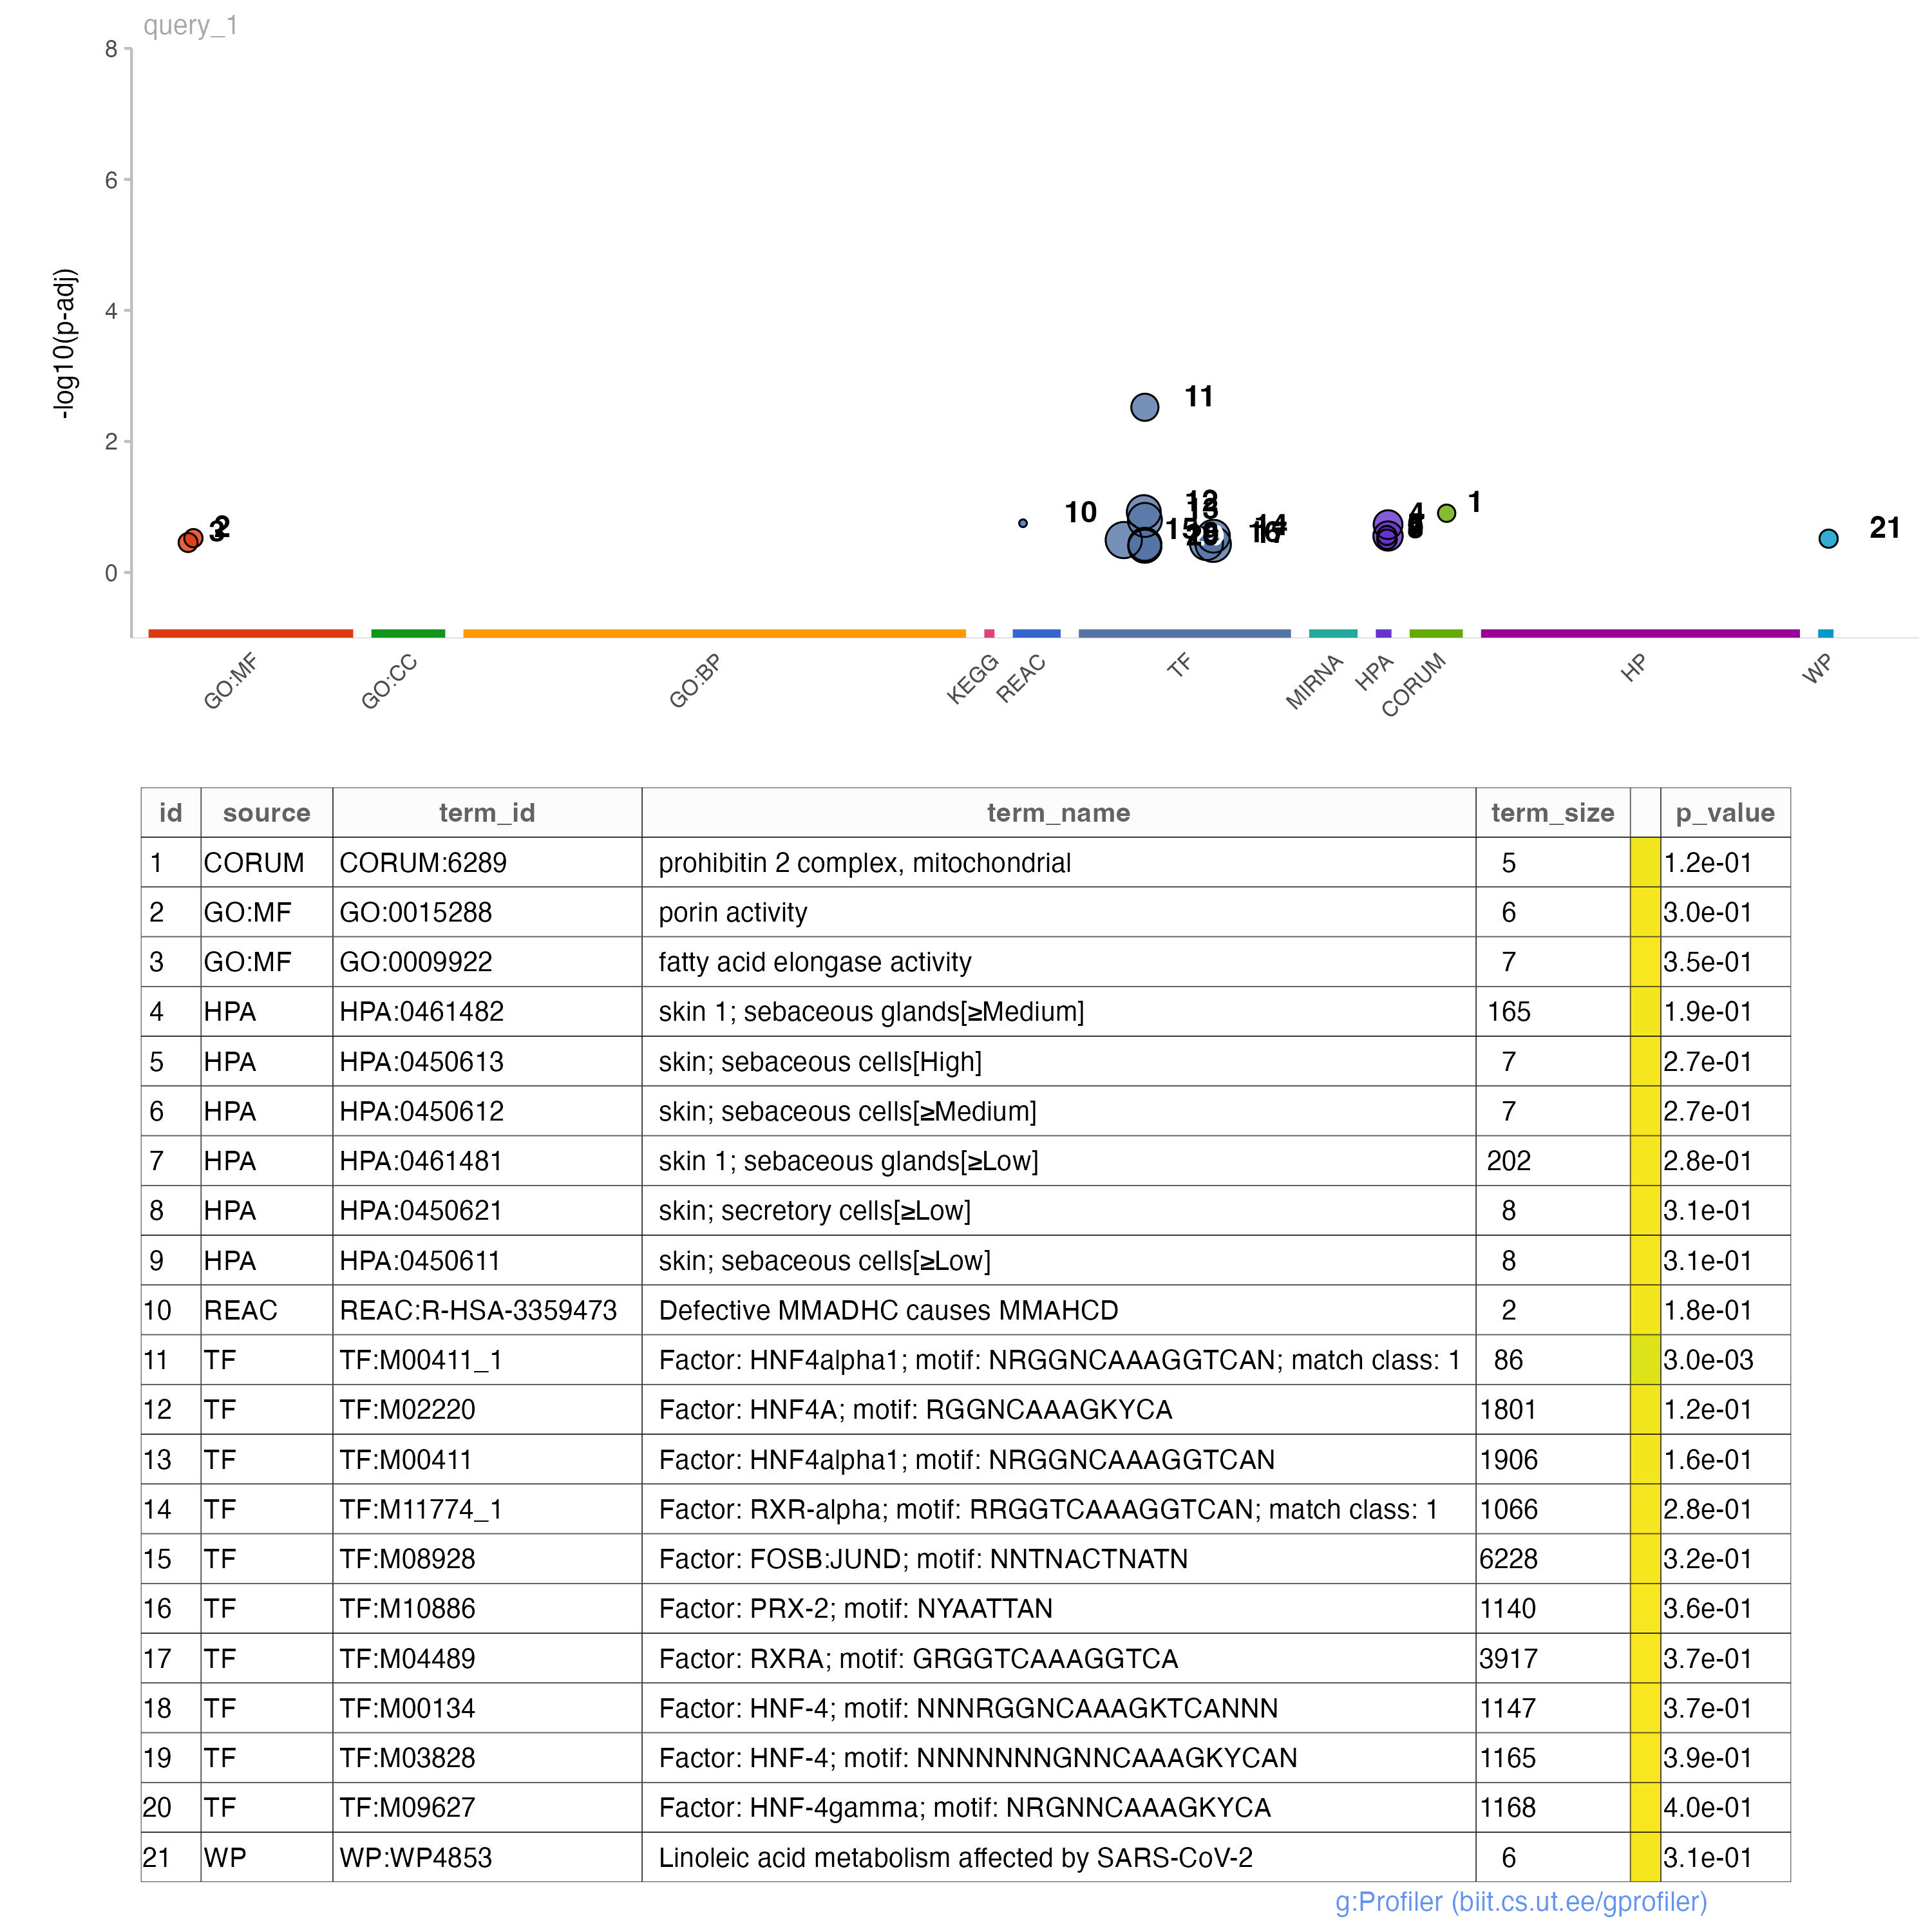
\includegraphics[width=1\linewidth]{images/demo_gostplot_mhplot_with_table} \end{center}

\begin{Shaded}
\begin{Highlighting}[]
\CommentTok{\# Assign gprofiler results}
\NormalTok{result\_df }\OtherTok{\textless{}{-}}\NormalTok{ gprofiler\_results}\SpecialCharTok{$}\NormalTok{result}

\CommentTok{\# Filter for significant results}
\NormalTok{significant\_gprofiler\_results }\OtherTok{\textless{}{-}}\NormalTok{ result\_df[result\_df}\SpecialCharTok{$}\NormalTok{significant, ]}

\CommentTok{\# Create a new column for {-}log10(p{-}value)}
\NormalTok{significant\_gprofiler\_results}\SpecialCharTok{$}\NormalTok{log\_p\_value }\OtherTok{\textless{}{-}} \SpecialCharTok{{-}}\FunctionTok{log10}\NormalTok{(significant\_results}\SpecialCharTok{$}\NormalTok{p\_value)}

\CommentTok{\# Print significant gprofiler results:}
\FunctionTok{print}\NormalTok{(significant\_gprofiler\_results)}

\CommentTok{\# Plot significant gProfiler results}
\FunctionTok{library}\NormalTok{(ggplot2)}
\NormalTok{signif\_gprofiler\_resplot }\OtherTok{\textless{}{-}} \FunctionTok{ggplot}\NormalTok{(}
\NormalTok{                                significant\_gprofiler\_results, }
                                \FunctionTok{aes}\NormalTok{(}\AttributeTok{x =} \FunctionTok{reorder}\NormalTok{(term\_name, log\_p\_value), }
                                    \AttributeTok{y =}\NormalTok{ log\_p\_value)) }\SpecialCharTok{+}
                                \FunctionTok{geom\_bar}\NormalTok{(}\AttributeTok{stat =} \StringTok{"identity"}\NormalTok{) }\SpecialCharTok{+}
                                \FunctionTok{theme\_minimal}\NormalTok{() }\SpecialCharTok{+}
                                \FunctionTok{coord\_flip}\NormalTok{() }\SpecialCharTok{+}
                                \FunctionTok{labs}\NormalTok{(}\AttributeTok{x =} \StringTok{"Enriched Terms"}\NormalTok{, }\AttributeTok{y =} \StringTok{"{-}log10(p{-}value)"}\NormalTok{, }
                                    \AttributeTok{title =} \StringTok{"Enrichment Analysis Results from gProfiler"}\NormalTok{) }\SpecialCharTok{+}
                                \FunctionTok{theme}\NormalTok{(}\AttributeTok{axis.text.x =} \FunctionTok{element\_text}\NormalTok{(}\AttributeTok{angle =} \DecValTok{45}\NormalTok{, }\AttributeTok{hjust =} \DecValTok{1}\NormalTok{)}
\NormalTok{                                ) }

\FunctionTok{print}\NormalTok{(signif\_gprofiler\_resplot)}
\end{Highlighting}
\end{Shaded}

\begin{center}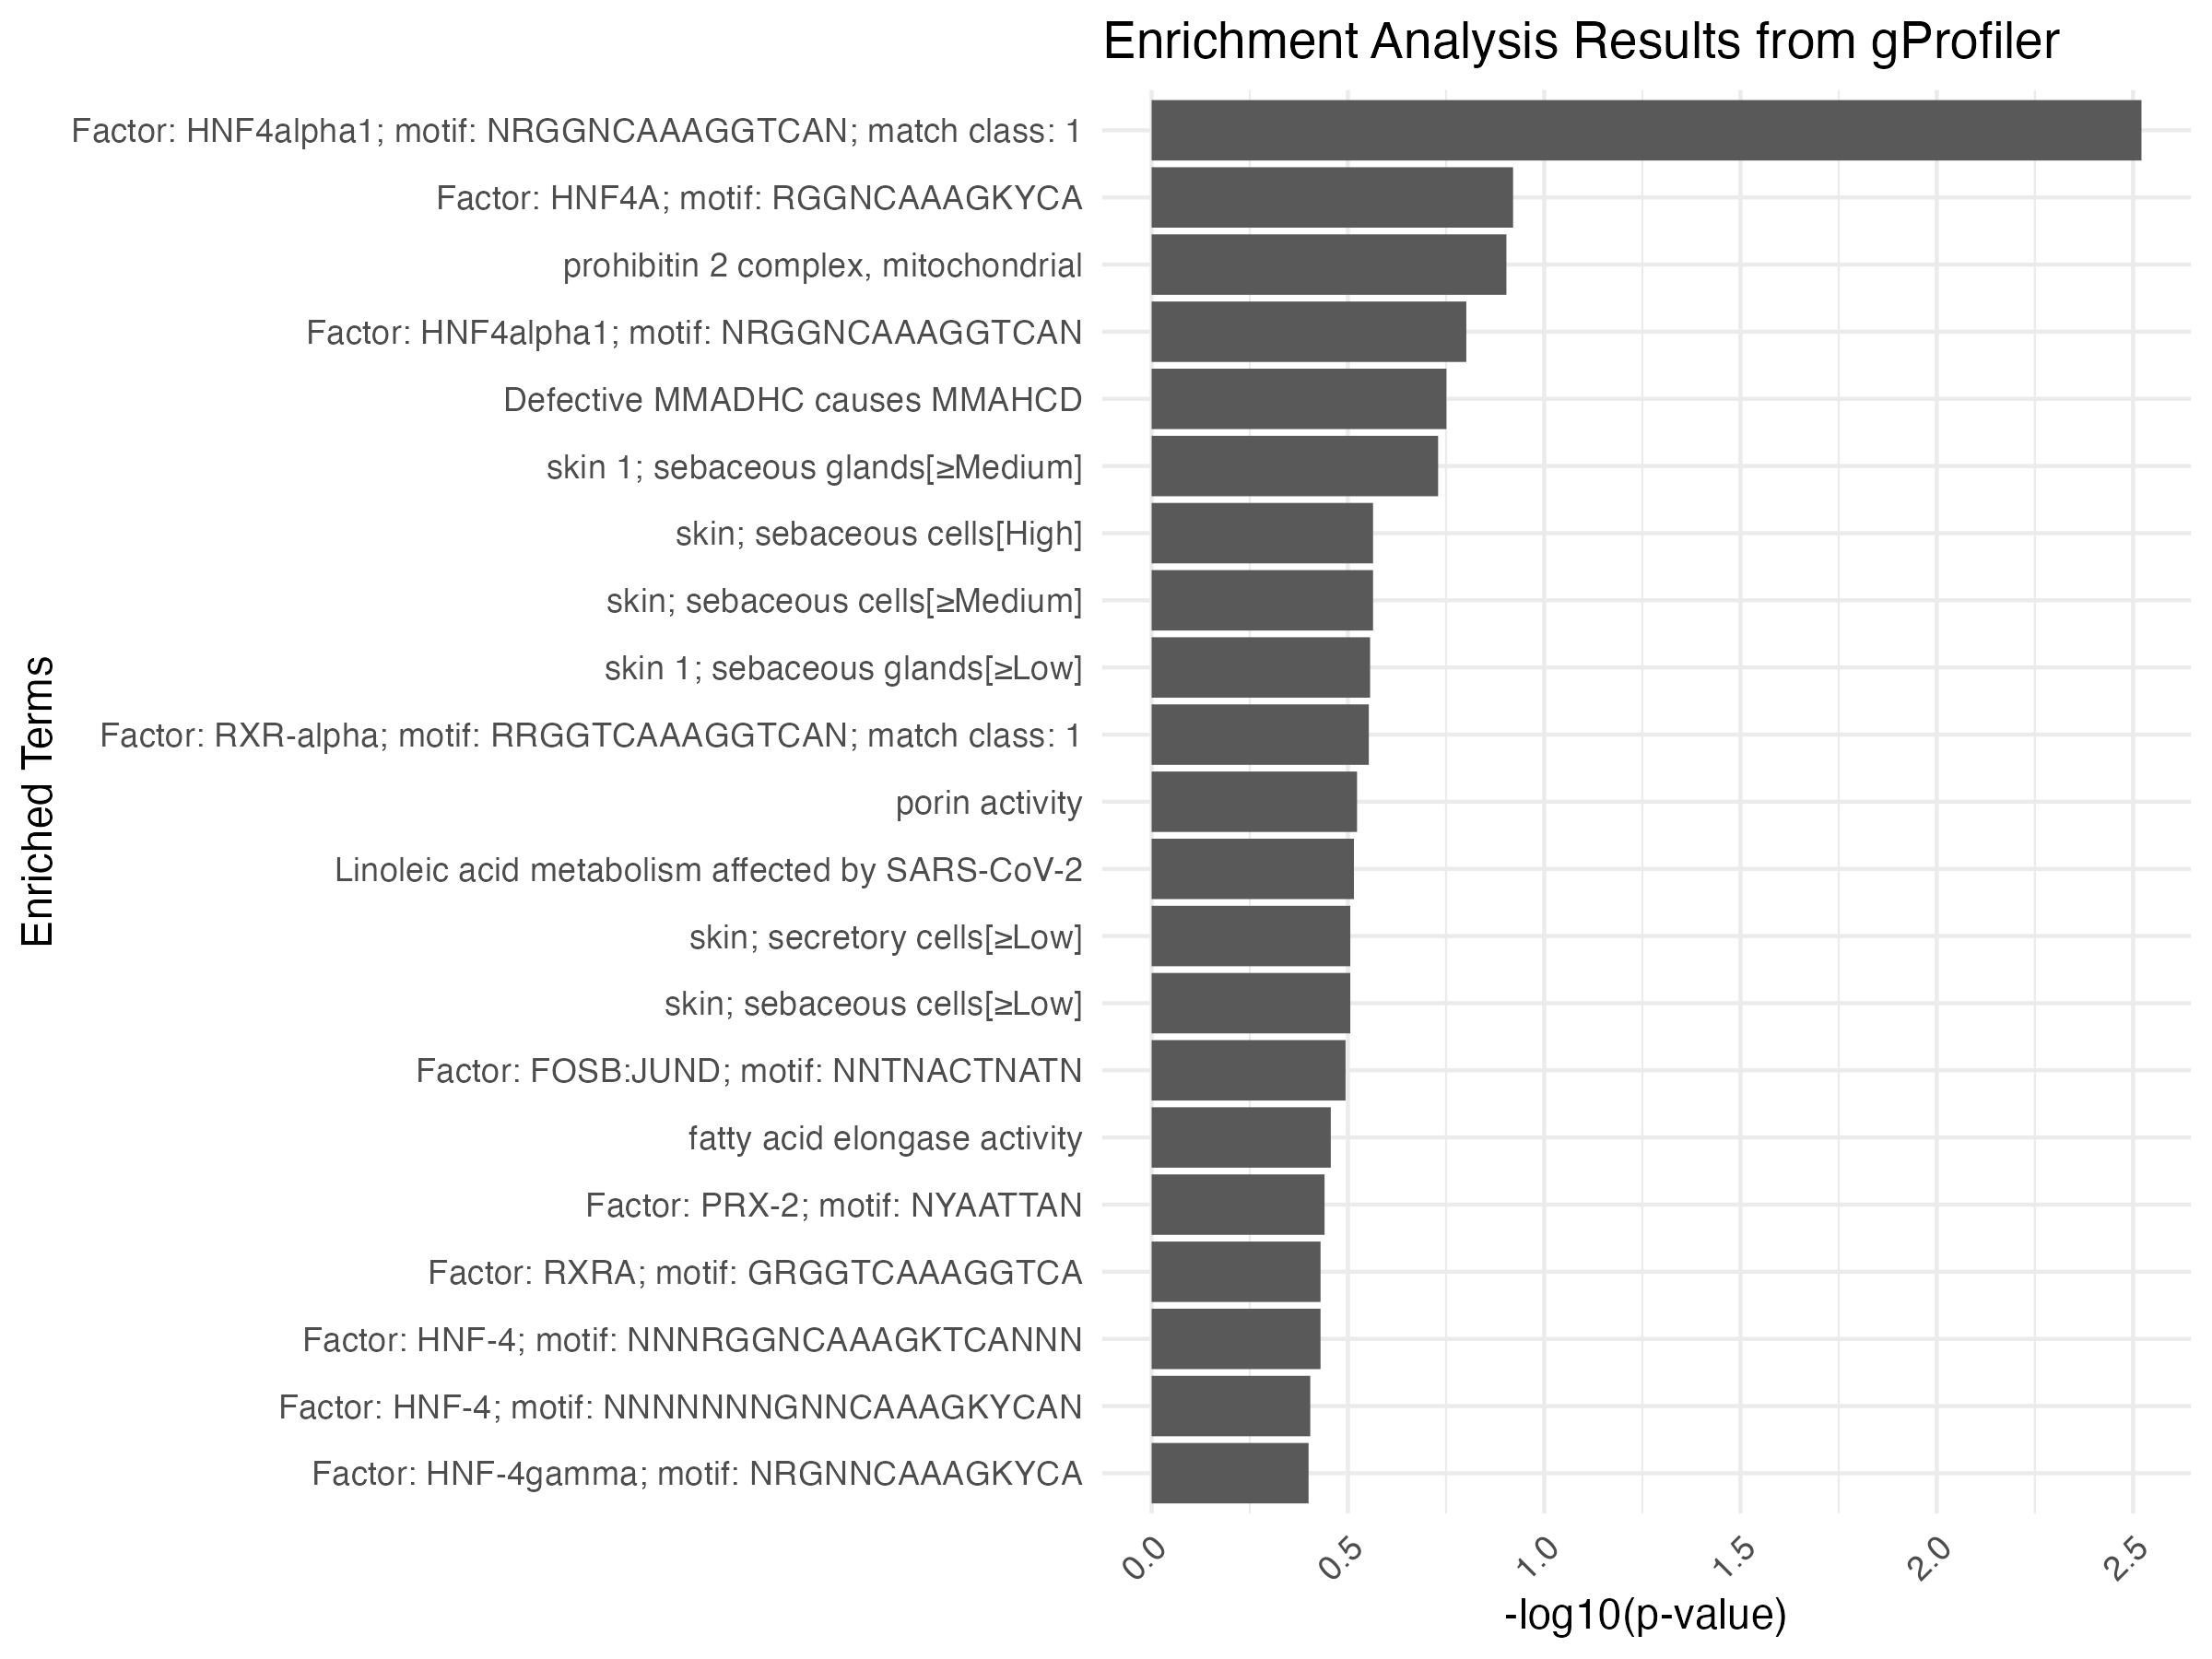
\includegraphics[width=1\linewidth]{images/demo_signif_gprofiler_resplot} \end{center}

\hypertarget{conclusion}{%
\section{Conclusion}\label{conclusion}}

Rf2pval provides comprehensive tools for bioinformatics analysis,
including features for machine learning, feature importance evaluation,
and more. This vignette covers the basics to get you started. For more
detailed documentation on the use of each function, please refer to the
function help pages within the package using the ?Rf2pval feature.

This package was created by Tyler Kolisnik, with support and assistance
from Dr.~Olin Silander, Dr.~Adam Smith \& Faeze Keshavarz.

Webpage: \url{www.github.com/tkolisnik/Rf2pval}.

Contact:
\href{mailto:tkolisnik@gmail.com}{\nolinkurl{tkolisnik@gmail.com}}

\end{document}
